% Options for packages loaded elsewhere
\PassOptionsToPackage{unicode}{hyperref}
\PassOptionsToPackage{hyphens}{url}
\PassOptionsToPackage{dvipsnames,svgnames,x11names}{xcolor}
%
\documentclass[
  a4paper,
  DIV=11,
  numbers=noendperiod,
  oneside]{scrreprt}

\usepackage{amsmath,amssymb}
\usepackage{iftex}
\ifPDFTeX
  \usepackage[T1]{fontenc}
  \usepackage[utf8]{inputenc}
  \usepackage{textcomp} % provide euro and other symbols
\else % if luatex or xetex
  \usepackage{unicode-math}
  \defaultfontfeatures{Scale=MatchLowercase}
  \defaultfontfeatures[\rmfamily]{Ligatures=TeX,Scale=1}
\fi
\usepackage{lmodern}
\ifPDFTeX\else  
    % xetex/luatex font selection
\fi
% Use upquote if available, for straight quotes in verbatim environments
\IfFileExists{upquote.sty}{\usepackage{upquote}}{}
\IfFileExists{microtype.sty}{% use microtype if available
  \usepackage[]{microtype}
  \UseMicrotypeSet[protrusion]{basicmath} % disable protrusion for tt fonts
}{}
\makeatletter
\@ifundefined{KOMAClassName}{% if non-KOMA class
  \IfFileExists{parskip.sty}{%
    \usepackage{parskip}
  }{% else
    \setlength{\parindent}{0pt}
    \setlength{\parskip}{6pt plus 2pt minus 1pt}}
}{% if KOMA class
  \KOMAoptions{parskip=half}}
\makeatother
\usepackage{xcolor}
\usepackage[left=1in,marginparwidth=2.0in,textwidth=4.0in,marginparsep=0.3in]{geometry}
\setlength{\emergencystretch}{3em} % prevent overfull lines
\setcounter{secnumdepth}{5}
% Make \paragraph and \subparagraph free-standing
\ifx\paragraph\undefined\else
  \let\oldparagraph\paragraph
  \renewcommand{\paragraph}[1]{\oldparagraph{#1}\mbox{}}
\fi
\ifx\subparagraph\undefined\else
  \let\oldsubparagraph\subparagraph
  \renewcommand{\subparagraph}[1]{\oldsubparagraph{#1}\mbox{}}
\fi


\providecommand{\tightlist}{%
  \setlength{\itemsep}{0pt}\setlength{\parskip}{0pt}}\usepackage{longtable,booktabs,array}
\usepackage{calc} % for calculating minipage widths
% Correct order of tables after \paragraph or \subparagraph
\usepackage{etoolbox}
\makeatletter
\patchcmd\longtable{\par}{\if@noskipsec\mbox{}\fi\par}{}{}
\makeatother
% Allow footnotes in longtable head/foot
\IfFileExists{footnotehyper.sty}{\usepackage{footnotehyper}}{\usepackage{footnote}}
\makesavenoteenv{longtable}
\usepackage{graphicx}
\makeatletter
\def\maxwidth{\ifdim\Gin@nat@width>\linewidth\linewidth\else\Gin@nat@width\fi}
\def\maxheight{\ifdim\Gin@nat@height>\textheight\textheight\else\Gin@nat@height\fi}
\makeatother
% Scale images if necessary, so that they will not overflow the page
% margins by default, and it is still possible to overwrite the defaults
% using explicit options in \includegraphics[width, height, ...]{}
\setkeys{Gin}{width=\maxwidth,height=\maxheight,keepaspectratio}
% Set default figure placement to htbp
\makeatletter
\def\fps@figure{htbp}
\makeatother
\newlength{\cslhangindent}
\setlength{\cslhangindent}{1.5em}
\newlength{\csllabelwidth}
\setlength{\csllabelwidth}{3em}
\newlength{\cslentryspacingunit} % times entry-spacing
\setlength{\cslentryspacingunit}{\parskip}
\newenvironment{CSLReferences}[2] % #1 hanging-ident, #2 entry spacing
 {% don't indent paragraphs
  \setlength{\parindent}{0pt}
  % turn on hanging indent if param 1 is 1
  \ifodd #1
  \let\oldpar\par
  \def\par{\hangindent=\cslhangindent\oldpar}
  \fi
  % set entry spacing
  \setlength{\parskip}{#2\cslentryspacingunit}
 }%
 {}
\usepackage{calc}
\newcommand{\CSLBlock}[1]{#1\hfill\break}
\newcommand{\CSLLeftMargin}[1]{\parbox[t]{\csllabelwidth}{#1}}
\newcommand{\CSLRightInline}[1]{\parbox[t]{\linewidth - \csllabelwidth}{#1}\break}
\newcommand{\CSLIndent}[1]{\hspace{\cslhangindent}#1}

\KOMAoption{captions}{tableheading}
\makeatletter
\@ifpackageloaded{tcolorbox}{}{\usepackage[skins,breakable]{tcolorbox}}
\@ifpackageloaded{fontawesome5}{}{\usepackage{fontawesome5}}
\definecolor{quarto-callout-color}{HTML}{909090}
\definecolor{quarto-callout-note-color}{HTML}{0758E5}
\definecolor{quarto-callout-important-color}{HTML}{CC1914}
\definecolor{quarto-callout-warning-color}{HTML}{EB9113}
\definecolor{quarto-callout-tip-color}{HTML}{00A047}
\definecolor{quarto-callout-caution-color}{HTML}{FC5300}
\definecolor{quarto-callout-color-frame}{HTML}{acacac}
\definecolor{quarto-callout-note-color-frame}{HTML}{4582ec}
\definecolor{quarto-callout-important-color-frame}{HTML}{d9534f}
\definecolor{quarto-callout-warning-color-frame}{HTML}{f0ad4e}
\definecolor{quarto-callout-tip-color-frame}{HTML}{02b875}
\definecolor{quarto-callout-caution-color-frame}{HTML}{fd7e14}
\makeatother
\makeatletter
\makeatother
\makeatletter
\@ifpackageloaded{bookmark}{}{\usepackage{bookmark}}
\makeatother
\makeatletter
\@ifpackageloaded{caption}{}{\usepackage{caption}}
\AtBeginDocument{%
\ifdefined\contentsname
  \renewcommand*\contentsname{Table of contents}
\else
  \newcommand\contentsname{Table of contents}
\fi
\ifdefined\listfigurename
  \renewcommand*\listfigurename{List of Figures}
\else
  \newcommand\listfigurename{List of Figures}
\fi
\ifdefined\listtablename
  \renewcommand*\listtablename{List of Tables}
\else
  \newcommand\listtablename{List of Tables}
\fi
\ifdefined\figurename
  \renewcommand*\figurename{Figure}
\else
  \newcommand\figurename{Figure}
\fi
\ifdefined\tablename
  \renewcommand*\tablename{Table}
\else
  \newcommand\tablename{Table}
\fi
}
\@ifpackageloaded{float}{}{\usepackage{float}}
\floatstyle{ruled}
\@ifundefined{c@chapter}{\newfloat{codelisting}{h}{lop}}{\newfloat{codelisting}{h}{lop}[chapter]}
\floatname{codelisting}{Listing}
\newcommand*\listoflistings{\listof{codelisting}{List of Listings}}
\makeatother
\makeatletter
\@ifpackageloaded{caption}{}{\usepackage{caption}}
\@ifpackageloaded{subcaption}{}{\usepackage{subcaption}}
\makeatother
\makeatletter
\@ifpackageloaded{tcolorbox}{}{\usepackage[skins,breakable]{tcolorbox}}
\makeatother
\makeatletter
\@ifundefined{shadecolor}{\definecolor{shadecolor}{rgb}{.97, .97, .97}}
\makeatother
\makeatletter
\makeatother
\makeatletter
\@ifpackageloaded{sidenotes}{}{\usepackage{sidenotes}}
\@ifpackageloaded{marginnote}{}{\usepackage{marginnote}}
\makeatother
\makeatletter
\makeatother
\ifLuaTeX
  \usepackage{selnolig}  % disable illegal ligatures
\fi
\IfFileExists{bookmark.sty}{\usepackage{bookmark}}{\usepackage{hyperref}}
\IfFileExists{xurl.sty}{\usepackage{xurl}}{} % add URL line breaks if available
\urlstyle{same} % disable monospaced font for URLs
\hypersetup{
  pdftitle={Statistics for Business and Social Sciences},
  colorlinks=true,
  linkcolor={blue},
  filecolor={Maroon},
  citecolor={Blue},
  urlcolor={Blue},
  pdfcreator={LaTeX via pandoc}}

\title{Statistics for Business and Social Sciences}
\author{}
\date{}

\begin{document}
\maketitle
\ifdefined\Shaded\renewenvironment{Shaded}{\begin{tcolorbox}[boxrule=0pt, sharp corners, breakable, borderline west={3pt}{0pt}{shadecolor}, interior hidden, frame hidden, enhanced]}{\end{tcolorbox}}\fi

\renewcommand*\contentsname{Table of contents}
{
\hypersetup{linkcolor=}
\setcounter{tocdepth}{2}
\tableofcontents
}
\bookmarksetup{startatroot}

\hypertarget{welcome}{%
\chapter*{Welcome}\label{welcome}}
\addcontentsline{toc}{chapter}{Welcome}

\markboth{Welcome}{Welcome}

Welcome to \textbf{Statistics for Business and Social Sciences}, a
comprehensive guide to understanding and harnessing the power of
statistics in the context of business and the social sciences. This
preface serves as an introduction to the rich and practical content that
you are about to embark upon.

In a world increasingly driven by data and information, the ability to
make sense of statistics is an invaluable skill. This course has been
designed to provide students with the fundamental tools and knowledge
necessary to not only understand statistics but also to apply them to
real-world problems in business and social sciences. Whether you are a
student, a professional, or simply someone interested in the world of
data, this course will equip you with the essential skills to navigate
the statistical landscape.

\textbf{Course Information}

At the heart of this course lies the commitment to empower students with
the ability to:

\begin{enumerate}
\def\labelenumi{\arabic{enumi}.}
\item
  \textbf{Describe the concepts} involved in solving problems related to
  statistics for business and social sciences (C2).
\item
  \textbf{Determine the appropriate methods} to address statistical
  problems encountered in business and social sciences (C5).
\item
  \textbf{Demonstrate interpersonal skills} through group work related
  to statistics for business and social sciences (A3).
\end{enumerate}

As you dive into the course, these outcomes will become your guiding
beacons, helping you measure your progress and the depth of your
understanding.

\textbf{Course Description}

Our journey through the world of statistics will begin by introducing
you to the basic and intermediate methods of data analysis. You will
explore the realms of descriptive and inferential statistics, which
encompass numerical descriptive measures, estimation, hypothesis
testing, and various statistical techniques. A significant emphasis is
placed on practicality, which will be evident as you delve into the use
of statistical software and interpretation of output.

\textbf{Syllabus Content}

The course content is divided into five distinct chapters, each building
upon the foundation laid by the preceding one:

\begin{itemize}
\item
  \textbf{Chapter 1: Introduction to Statistics} provides the groundwork
  by defining what statistics is, explaining the types of variables,
  data, and methods of data collection.
\item
  \textbf{Chapter 2: Descriptive Statistics} explores the art of
  organizing data and calculating various measures of central tendency,
  variation, skewness, and position.
\item
  \textbf{Chapter 3: Estimation} delves into the concept of sampling
  distribution and interval estimation for means, both for independent
  and dependent samples.
\item
  \textbf{Chapter 4: Hypothesis Testing} equips you with the skills
  needed to test hypotheses about means and variances in various
  scenarios, including one-way analysis of variance and testing for
  independence.
\item
  \textbf{Chapter 5: Bivariate Analysis} ventures into the world of
  relationships between variables, covering correlation, simple linear
  regression, and the estimation of linear regression using the least
  squares method.
\end{itemize}

Each chapter serves as a stepping stone, progressively building your
knowledge and competence in the world of statistics.

Throughout your journey, you'll find numerous examples, exercises, and
real-world applications to reinforce your understanding. Remember, this
course isn't just about theory; it's about practical skills that you can
apply to real-life situations.

We hope this course becomes your gateway to the world of statistics,
enabling you to approach business and social sciences with newfound
confidence and precision. So, fasten your seatbelts, embrace the
challenges, and get ready to embark on a statistical adventure that will
broaden your horizons and empower you with valuable skills.

\bookmarksetup{startatroot}

\hypertarget{preface}{%
\chapter*{Preface}\label{preface}}
\addcontentsline{toc}{chapter}{Preface}

\markboth{Preface}{Preface}

Welcome to ``Statistics for Business and Social Sciences.'' This book is
designed to be your comprehensive guide to the world of statistics,
tailored specifically to the curriculum of Universiti Teknologi MARA's
undergraduate program. Whether you are a business major, social sciences
enthusiast, or a student in any discipline, this book will equip you
with the essential knowledge and skills to harness the power of
statistics.

In the fast-paced and data-driven world we live in, the ability to make
informed decisions is paramount. Statistics is the language of data, and
its principles are woven into countless aspects of our daily lives.
Understanding statistics is not just an academic endeavor; it's a
practical tool that can empower you to navigate the complexities of your
chosen field.

The book begins with ``Introduction to Statistics,'' setting the stage
by exploring the fundamental concepts, the role of statistics in
research and decision-making, and the ethical considerations of data
analysis. We then delve into ``Descriptive Statistics,'' where we unveil
the art of summarizing and presenting data in a meaningful way.

``Estimation'' and ``Hypothesis Testing'' are two pivotal chapters that
bridge the gap between data and decision-making. You'll learn how to
make educated guesses about population parameters and how to rigorously
test hypotheses using real-world examples.

The journey culminates in ``Bivariate Analysis,'' where we explore the
relationships between two variables, offering insights into correlation,
regression, and their applications in business and social sciences.

Each chapter is designed with clarity in mind, with practical examples
and exercises to reinforce your understanding. Additionally, we provide
a range of resources, including data sets and online tools, to help you
apply your knowledge beyond the textbook.

As you embark on this statistical voyage, remember that learning
statistics is not just about mastering formulas and techniques; it's
about developing a critical mindset, where you can question, interpret,
and draw meaningful conclusions from data. This book is your trusted
companion in that journey.

We hope this book becomes an invaluable resource, both in your academic
pursuits and in your future professional endeavors. Embrace the world of
statistics with confidence, and discover how it can enhance your ability
to analyze, interpret, and contribute to the business and social
sciences fields.

Statistics may appear daunting at first, but with patience and
persistence, it can be a fascinating and empowering discipline. So,
let's embark on this enlightening journey together, and may this book be
your steadfast guide. Enjoy your exploration of ``Statistics for
Business and Social Sciences.''

Rosidah Ahmad

Kamarul Ariffin Mansor

Ida Normaya Mohd Nasir

Norin Rahayu Shamsuddin

\bookmarksetup{startatroot}

\hypertarget{introduction-to-statistics}{%
\chapter{Introduction to Statistics}\label{introduction-to-statistics}}

\hypertarget{learning-objectives}{%
\section*{Learning Objectives}\label{learning-objectives}}
\addcontentsline{toc}{section}{Learning Objectives}

\markright{Learning Objectives}

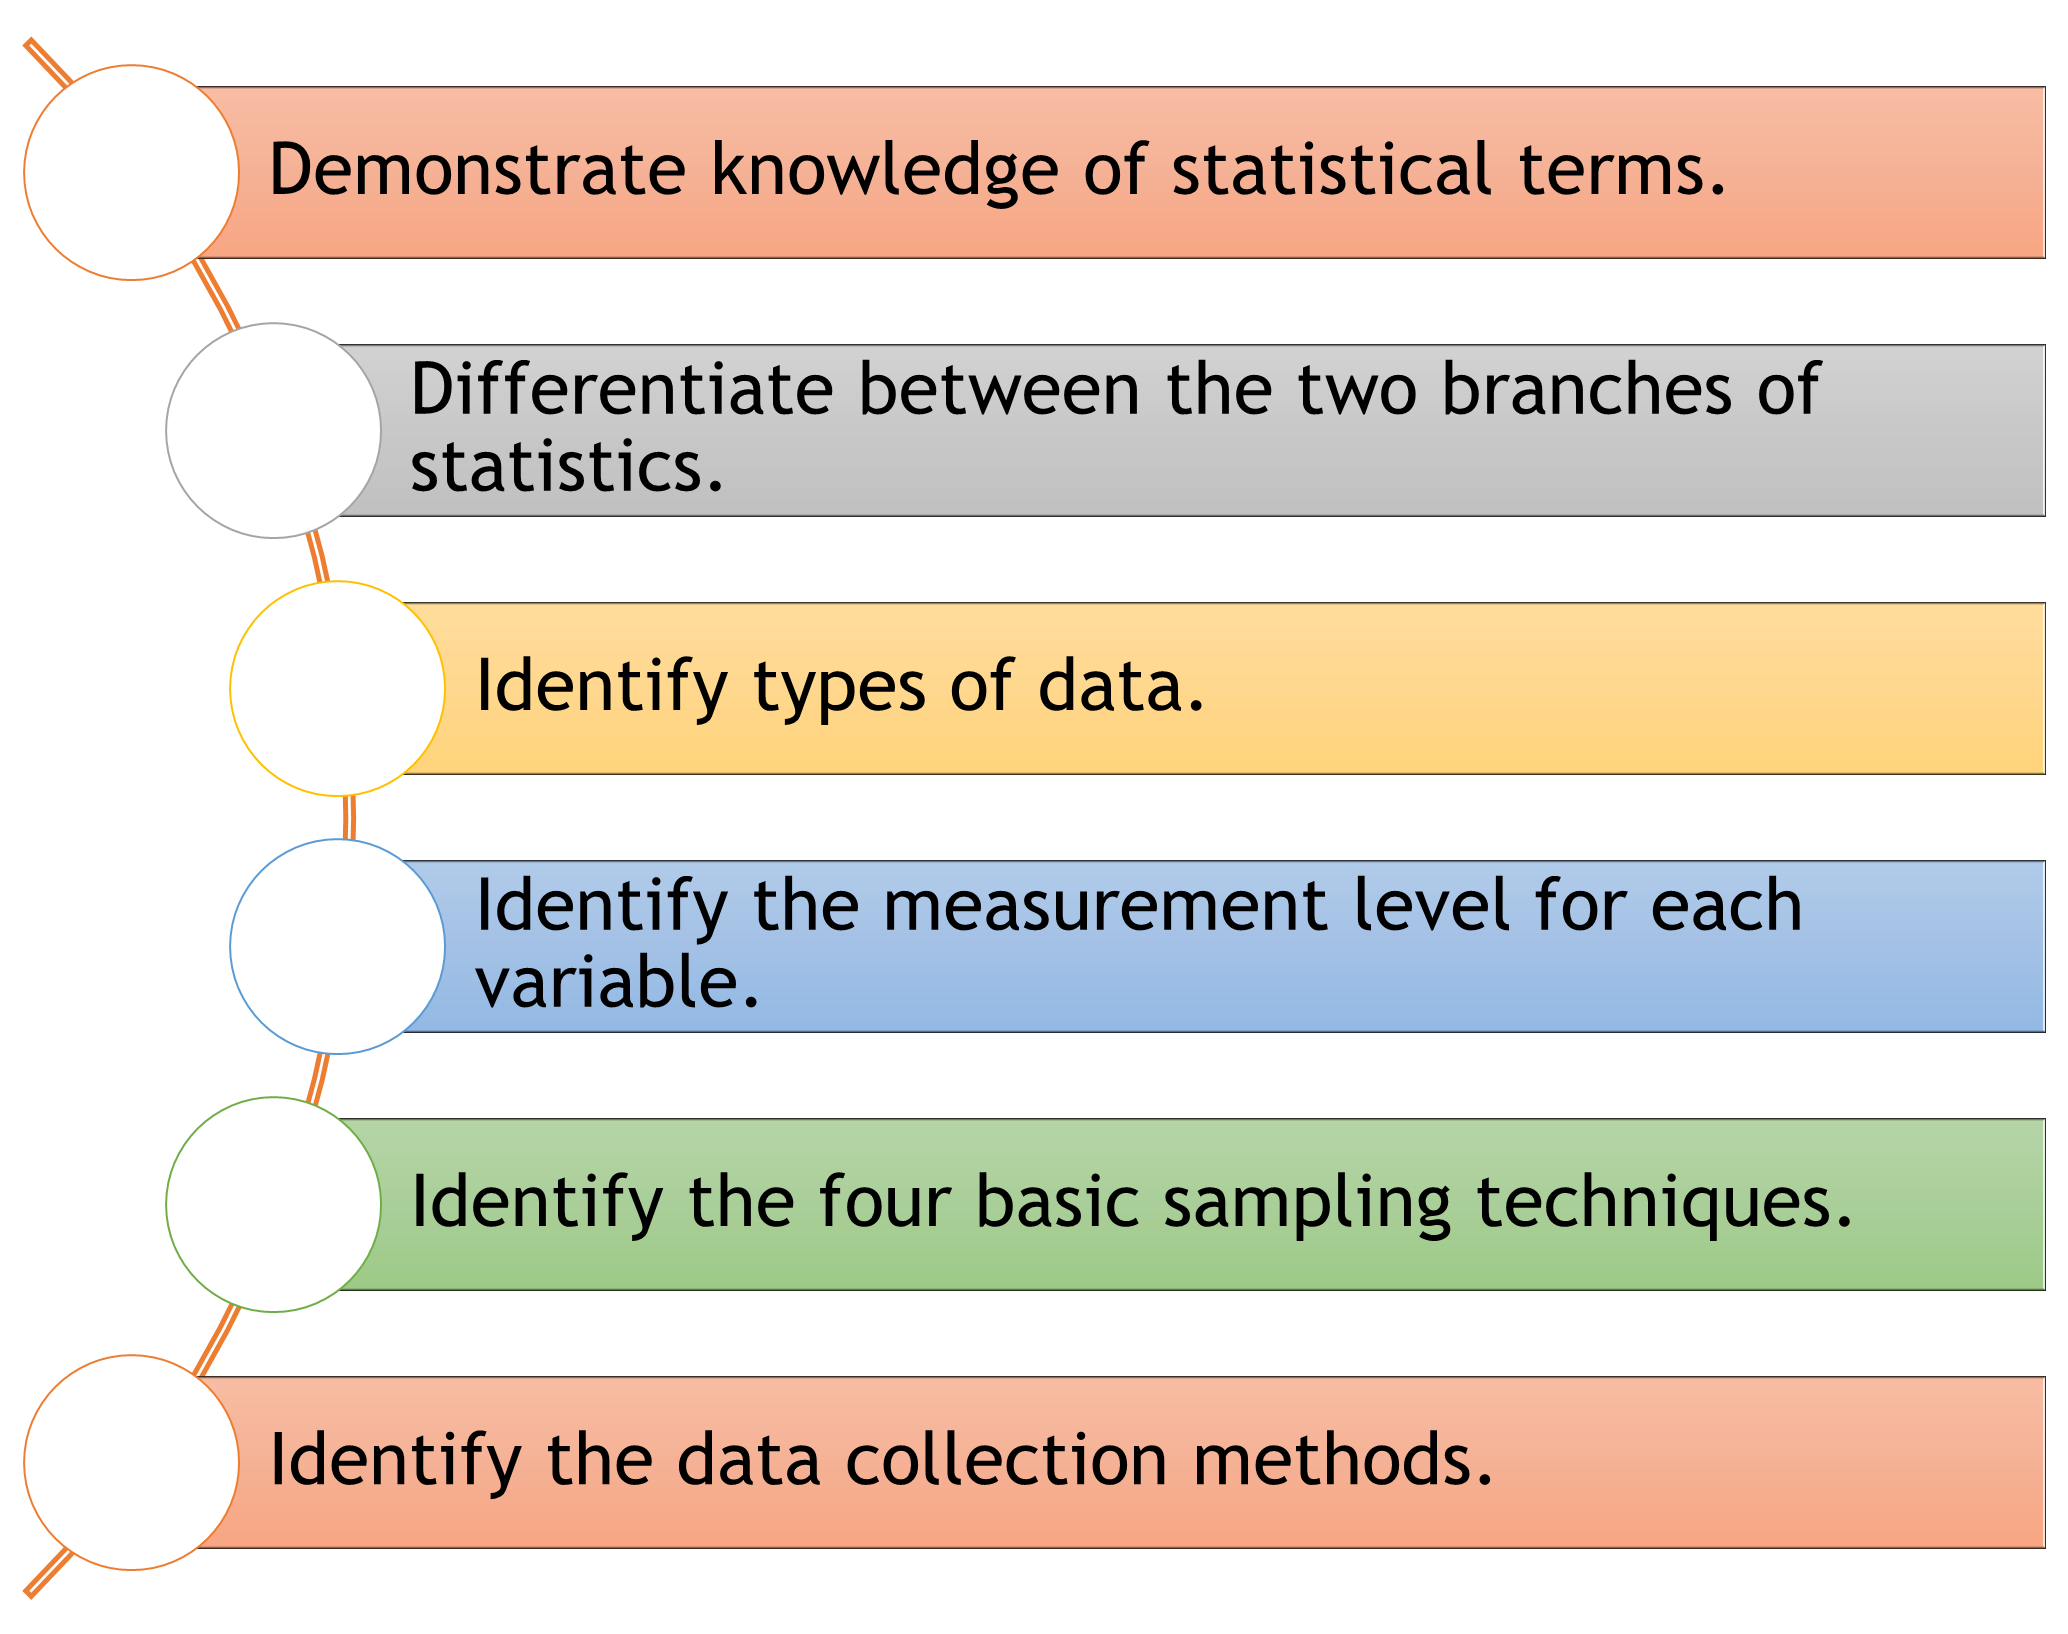
\includegraphics[width=6.25in,height=\textheight]{images/ch1/Picture1.png}

\hypertarget{introduction}{%
\section{\texorpdfstring{Introduction\\
}{Introduction }}\label{introduction}}

\textbf{Why study statistics?}\\

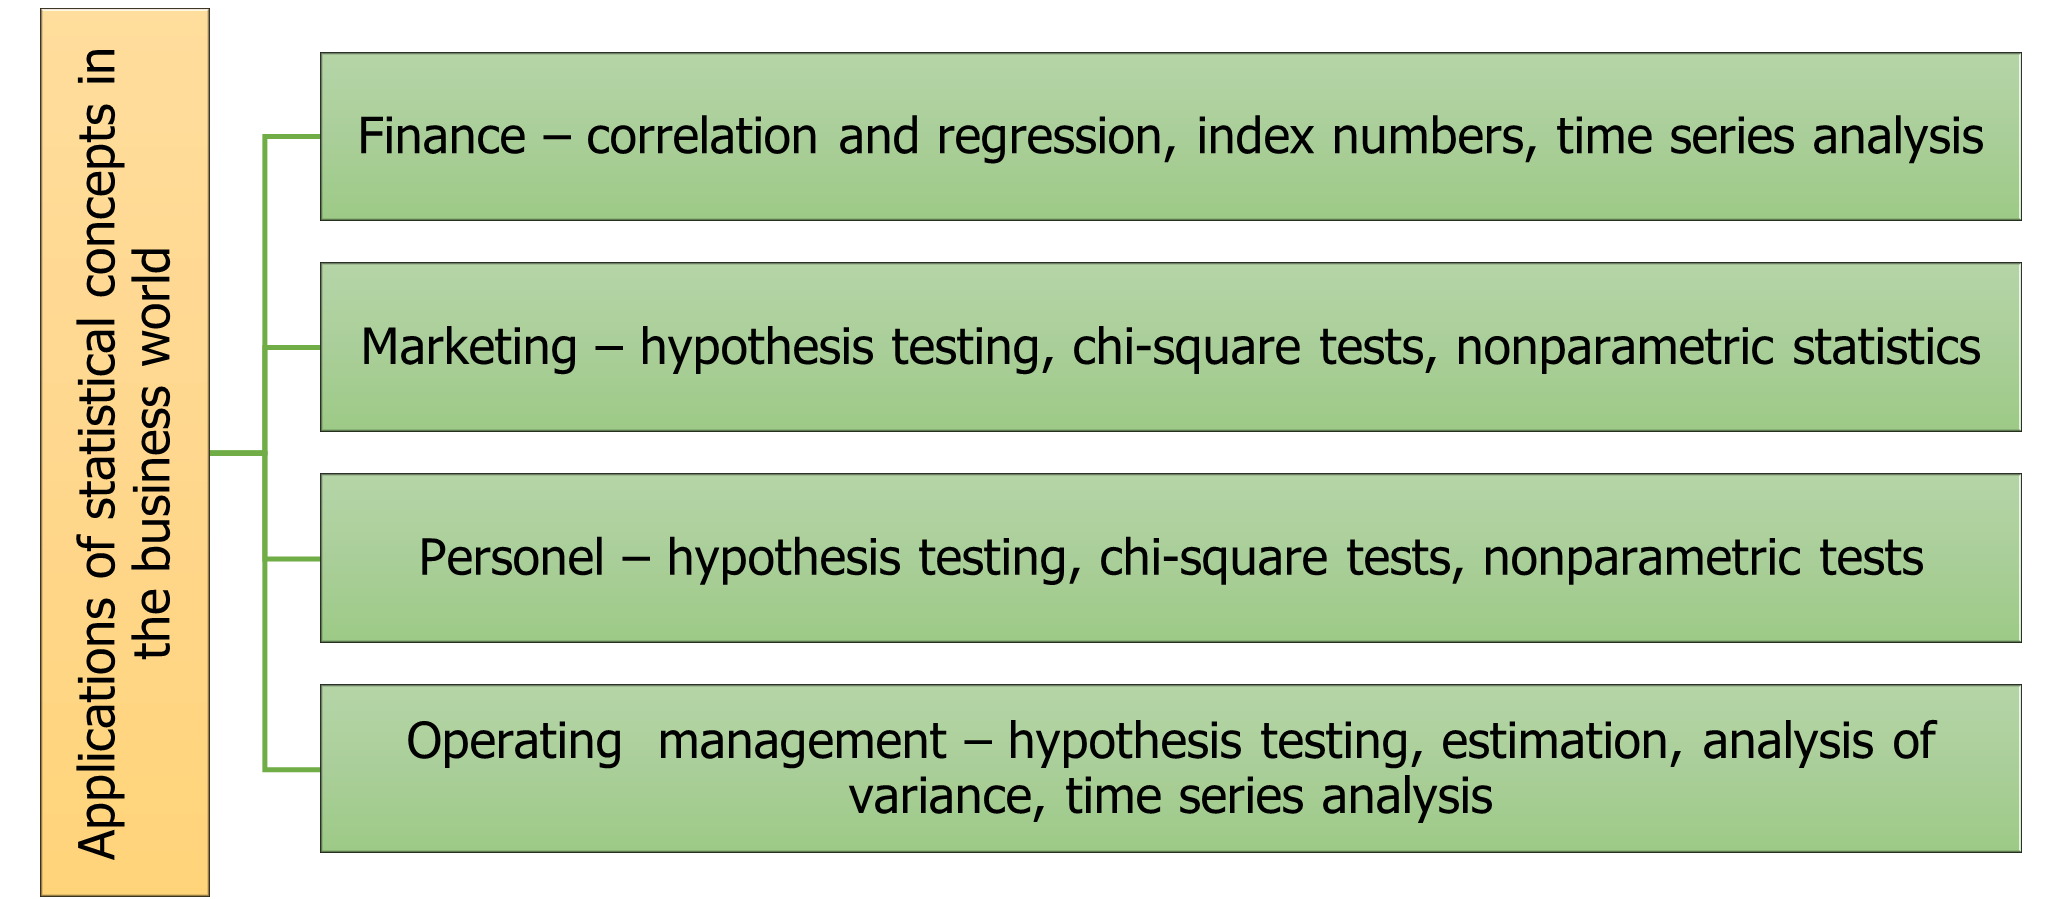
\includegraphics[width=6.25in,height=\textheight]{images/ch1/Picture2.png}

\hypertarget{what-is-statistics}{%
\section{\texorpdfstring{What is Statistics?\\
}{What is Statistics? }}\label{what-is-statistics}}

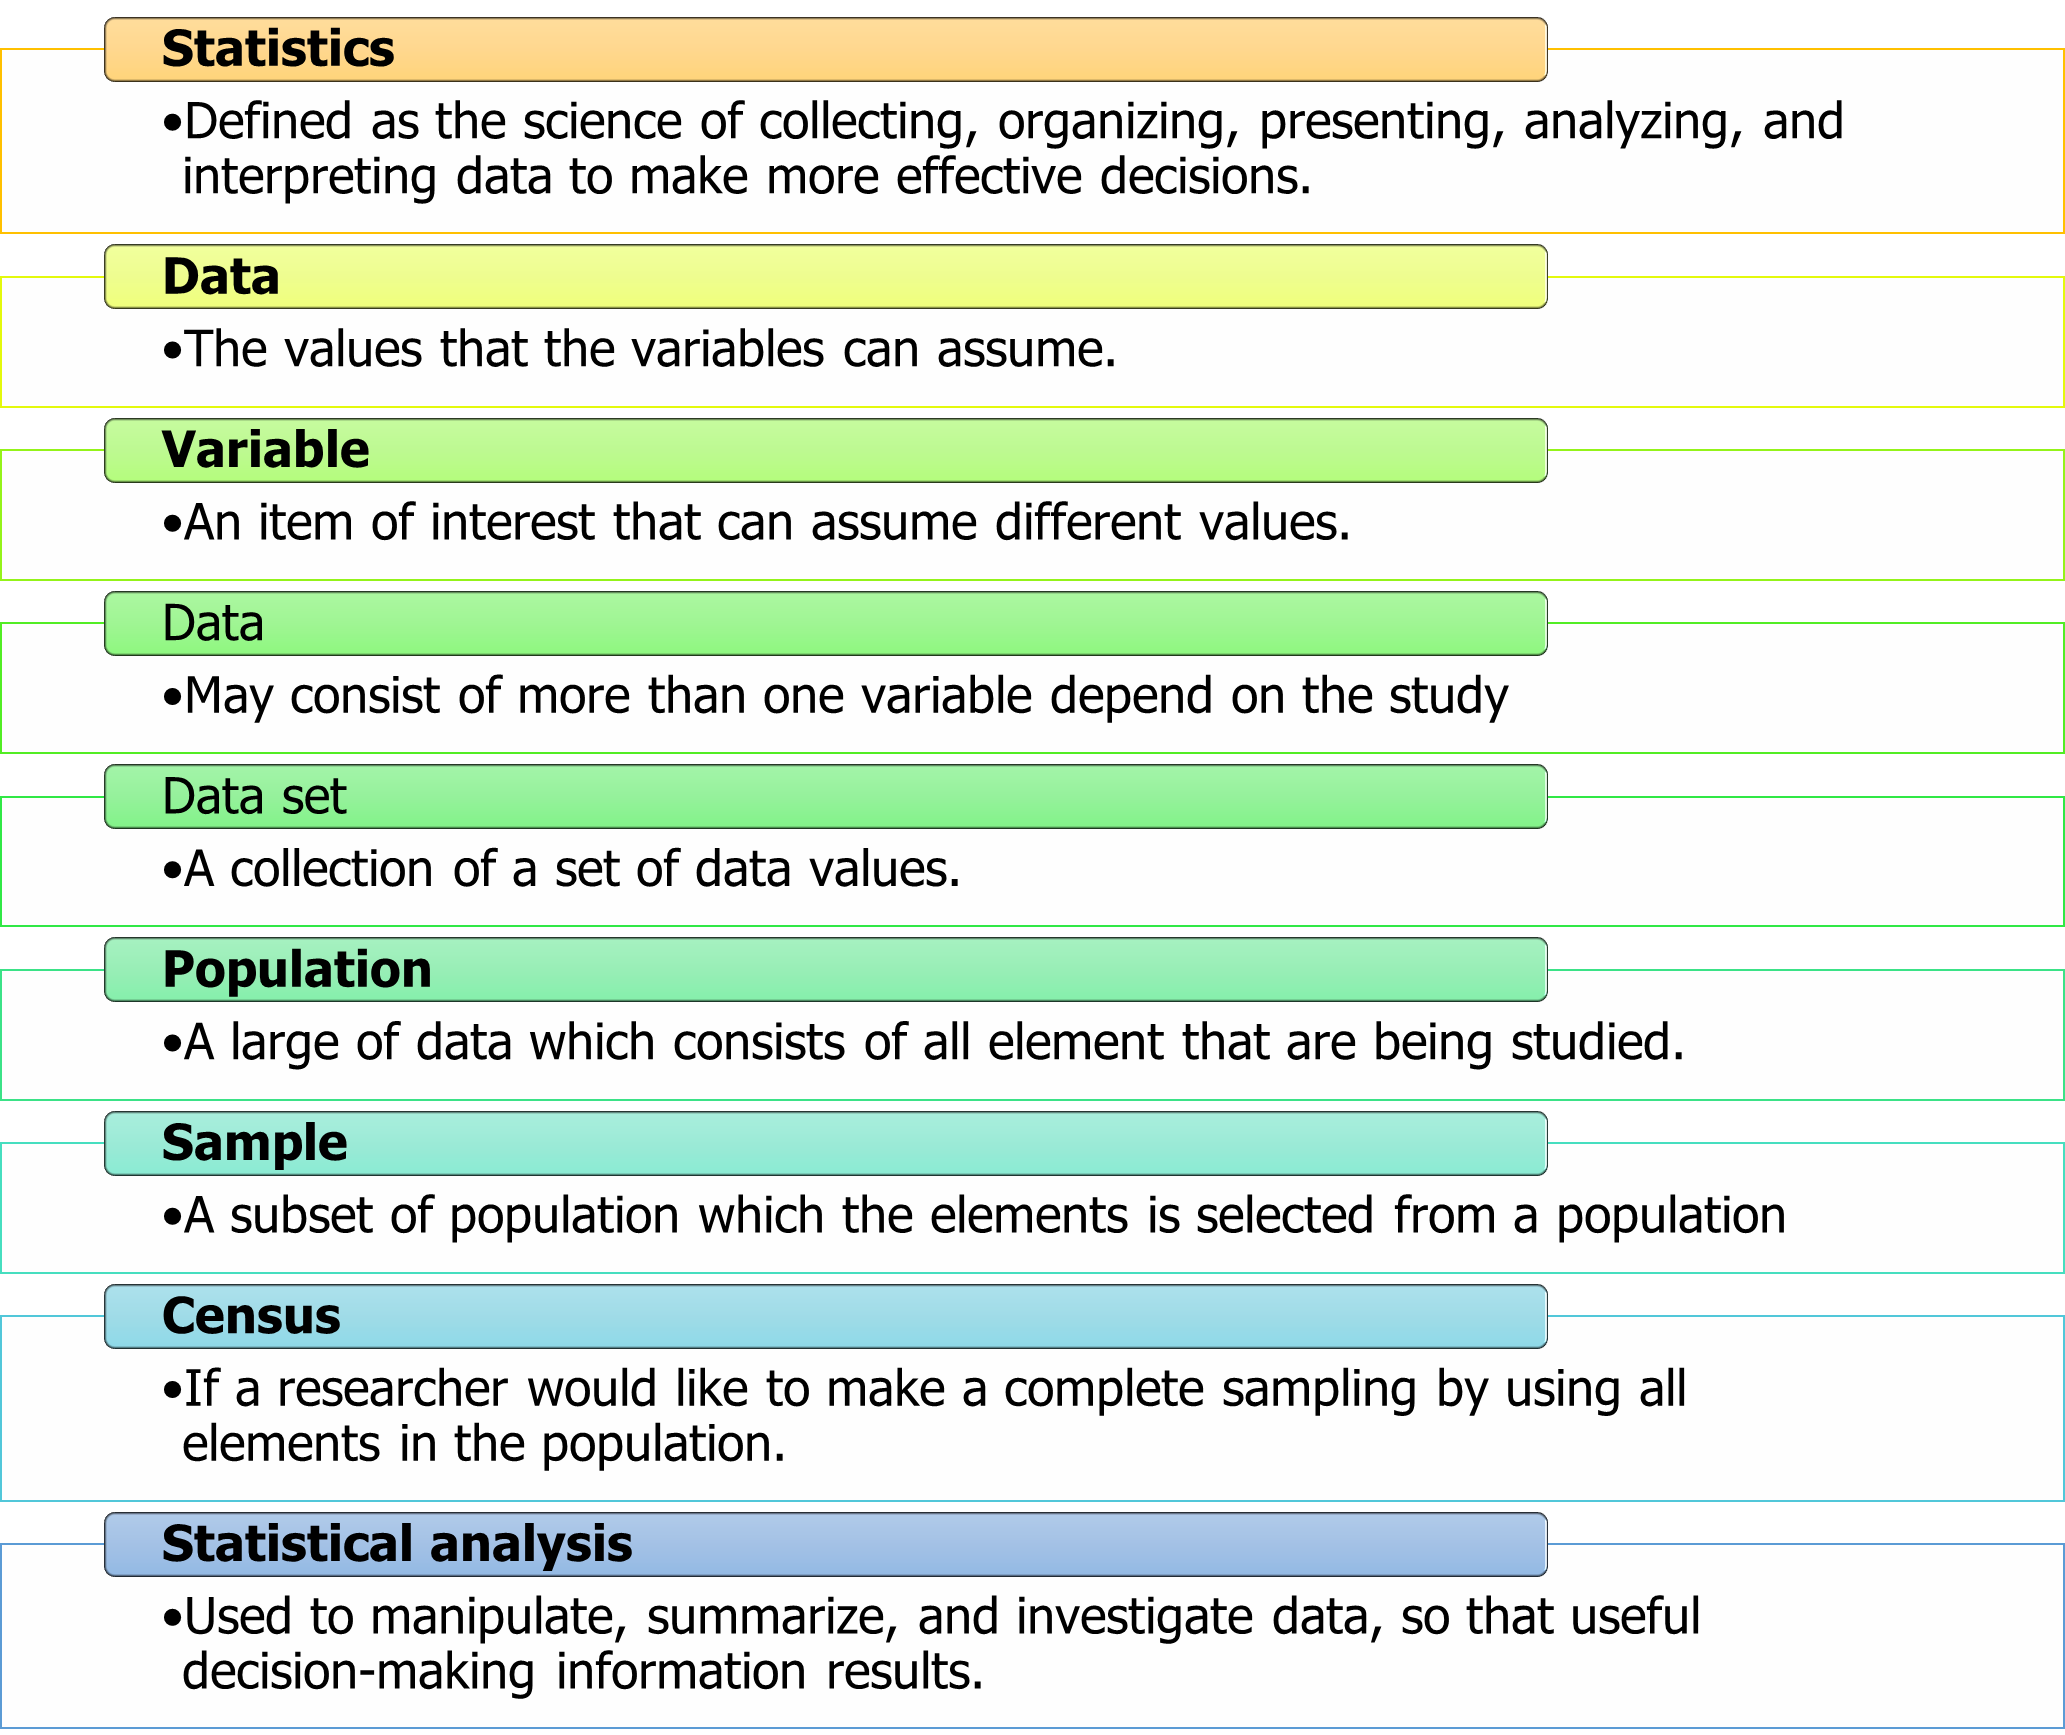
\includegraphics[width=6.25in,height=\textheight]{images/ch1/Picture3.png}

\begin{figure}

{\centering 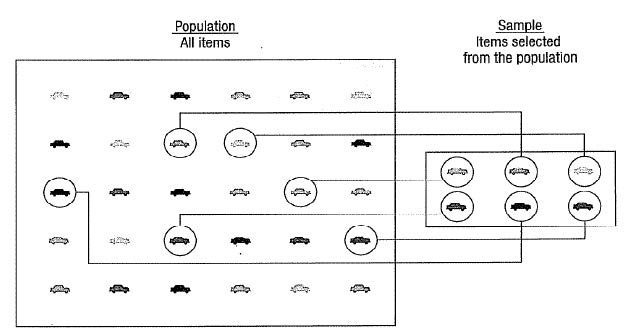
\includegraphics[width=5.20833in,height=\textheight]{images/ch1/Picture4.jpg}

}

\caption{Figure 1.1: Population and Sample}

\end{figure}

{\textbf{Example 1.1}}

Determine the population, sample, and variable(s).

\begin{enumerate}
\def\labelenumi{\alph{enumi})}
\item
  The Dean from College YY would like to determine students' performance
  through online distance learning (ODL). From 1000 students, the dean
  decides to select only 300 students as a respondent. The information
  about the number of hours spent and assessment marks are collected.
\item
  A headmaster of School Y conducted a study on students' satisfaction
  (strongly disagree=1, disagree=2, neutral=3, agree=4, strongly
  agree=5) with online distance learning conducted by their teachers.
  The headmaster selects only 10 out of 50 classes in School Y. The
  study included all students in these classes.
\end{enumerate}

{\textbf{Answer}}

\begin{enumerate}
\def\labelenumi{\alph{enumi})}
\item
  Population: All 1000 students from College YY. Sample: 300 students
  from College YY. Variable: i) Number of hours spent ii) Assessment
  marks
\item
  Population: All students from 50 classes of School Y. Sample: Students
  from selected 10 classes. Variable: Students' satisfaction
\end{enumerate}

\hypertarget{type-of-statistics}{%
\section{Type of statistics}\label{type-of-statistics}}

Generally, \textbf{statistics} is divided into two broad categories,
depending on how data are used. The two categories are
\textbf{Descriptive Statistics} and \textbf{Inferential Statistics}. A
\textbf{Descriptive Statistics} describe a \emph{summary} information
about variables in data. While, \textbf{Inferential Statistics} uses
sample data to make an inference or draw a conclusion about the
population. The description of Descriptive Statistics and Inferential
Statistics shown in Table 1.1.

\begin{figure}

{\centering 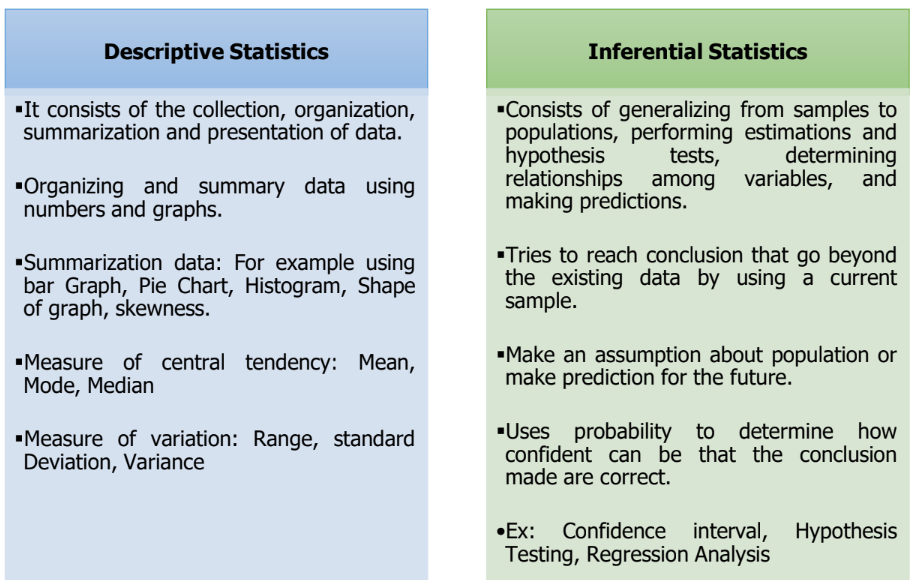
\includegraphics[width=5.20833in,height=\textheight]{images/ch1/Picture5.png}

}

\caption{Table 1.1 Descriptive Statistics and Inferential Statistics}

\end{figure}

{\textbf{Example 1.2}}

\begin{enumerate}
\def\labelenumi{\alph{enumi})}
\tightlist
\item
  The average donation received from Five Top Company was RM50000.
\item
  In a research study found that anxiety with behavioral intention has a
  significant inverse causal effect on the behavior of students using
  communication technology.
\end{enumerate}

{\textbf{Answer}}

\begin{enumerate}
\def\labelenumi{\alph{enumi})}
\tightlist
\item
  Descriptive Statistics
\item
  Inferential Statistics
\end{enumerate}

\hypertarget{type-of-data}{%
\section{Type of data}\label{type-of-data}}

The term ``Data'' refers to a collection of measurements made on one or
more observational units that used to describe situations or events.
Statistical data are usually obtained by counting or measuring items.
Depending on the sources, statistical data are classified into two
types; \textbf{Primary Data} and \textbf{Secondary Data}.

\begin{enumerate}
\def\labelenumi{\alph{enumi})}
\item
  \emph{Primary data} is a data that are collected for the first time
  and are thus original in nature.
\item
  \emph{Secondary data} have already been compiled or collected by some
  other persons and are available for statistical analysis.
\end{enumerate}

The advantages and disadvantages of primary and secondary data shown in
Table 1.2.

\begin{figure}

{\centering 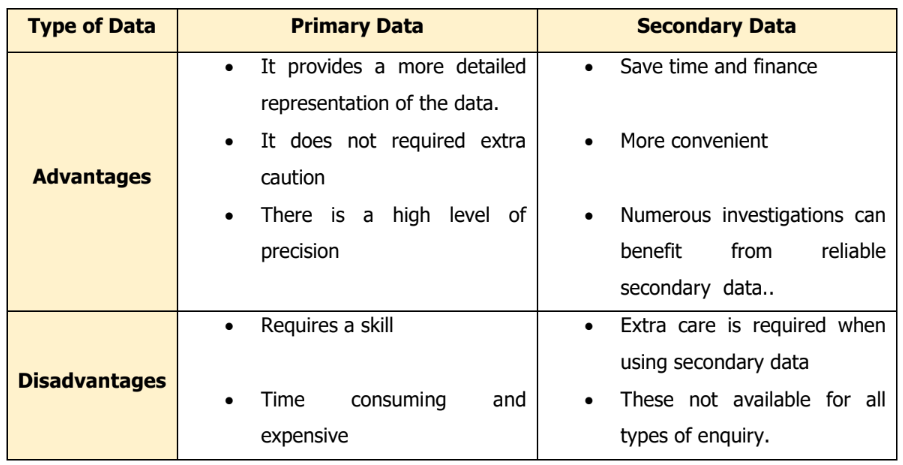
\includegraphics[width=5.20833in,height=\textheight]{images/ch1/Picture6.png}

}

\caption{Table 1.2 Advantages and disadvantage of primary and secondary
data}

\end{figure}

{\textbf{Example 1.3}}

Describe the type of data below.

\begin{enumerate}
\def\labelenumi{\alph{enumi})}
\tightlist
\item
  A statistics textbook
\item
  A mailed questionnaire
\end{enumerate}

{\textbf{Answer}}

\begin{enumerate}
\def\labelenumi{\alph{enumi})}
\tightlist
\item
  Secondary Data
\item
  Primary Data
\end{enumerate}

\hypertarget{data-collection}{%
\section{Data collection}\label{data-collection}}

Data are collected in a variety of ways. For \textbf{primary data}, one
of the most common method is through the use of survey. Survey is a
research process of collecting a data that can be done by using a
variety of method. The most common methods are telephone surveys,
questionnaire survey and the personal interviews. The descriptions of
these methods are shown in Table 1.3.

\begin{figure}

{\centering 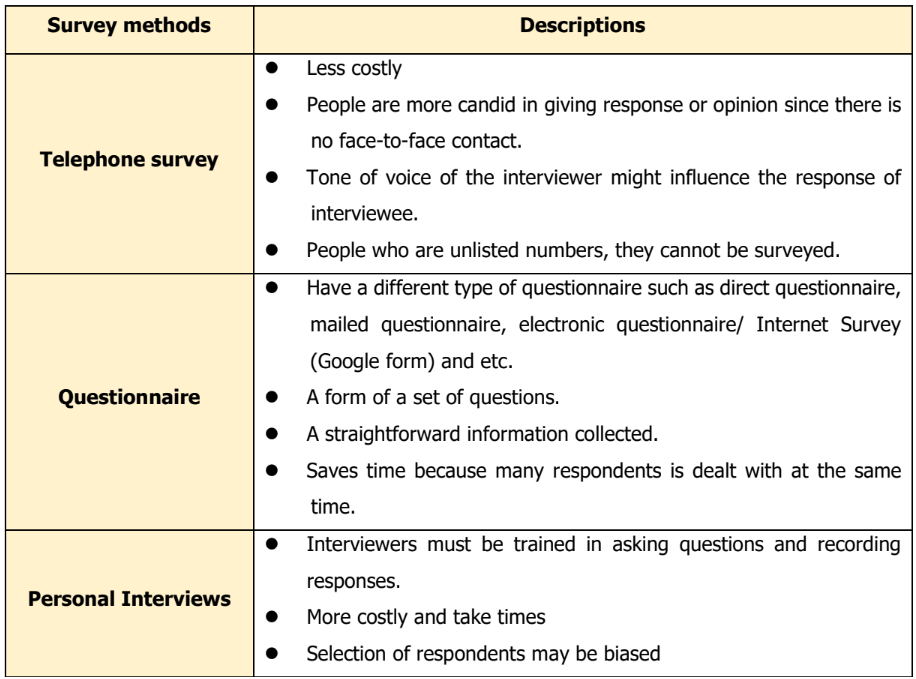
\includegraphics[width=5.20833in,height=\textheight]{images/ch1/Picture7.png}

}

\caption{Table 1.3 Descriptions of telephone surveys, questionnaire
survey and personal interviews}

\end{figure}

\textbf{Secondary data} are collected from readily available sources
such as websites, article journals, books, etc. It supplies second-hand
data collection from other sources, either from individuals or an
organization. Among the top sources of secondary data are:

\begin{enumerate}
\def\labelenumi{\alph{enumi})}
\tightlist
\item
  Journal articles that comment on or analyse research
\item
  Textbooks
\item
  Dictionaries and encyclopaedias
\item
  Book and interpret, analyse
\item
  Political commentary
\item
  Biographies
\item
  Dissertations
\item
  Newspaper editorial/opinion pieces
\end{enumerate}

\hypertarget{variables-and-types-of-variables}{%
\section{Variables and types of
variables}\label{variables-and-types-of-variables}}

Variables can be classified as Quantitative Variable or Qualitative
Variable.

\hypertarget{quantitative-variables}{%
\subsection{Quantitative Variables}\label{quantitative-variables}}

Quantitative data is an observation that are measured on a numerical
scale. Basically, the quantitative data are in the form of values,
percentage, frequency, or numbers. This type of data can be visualized
using diagram such as tables, graphs, and histogram.

If the variables in the data are being studied, the variables that are
report numerically is called quantitative variable.

Quantitative variables are always in numbers and are the result of
counting or measuring attributes of a population. Quantitative variable
can be separated into two subgroups:

\begin{quote}
\textbf{Discrete} can assume only integer value (if it is the result of
counting, examples the number of students of a given ethnic group in a
class, the number of books on a shelf)
\end{quote}

\begin{quote}
\textbf{Continuous} can assume any value over a continuous range of
possibilities (if it is the result of measuring, examples distance
traveled, weight of luggage)
\end{quote}

\hypertarget{qualitative-variables}{%
\subsection{Qualitative Variables}\label{qualitative-variables}}

Qualitative data is opposite with quantitative data. Qualitative data
provide varieties of items in terms of categories base. It is generally
described by words or letters. For example, in qualitative data may
contains information about gender, age category or pass or fail.However,
if the characteristics or variables being studied is in categorical or
non-numerical it is called as qualitative variable.

Qualitative variables can be separated into two subgroups:

\begin{quote}
\textbf{dichotomic} (if it takes the form of a word with two options
(gender - male or female)
\end{quote}

\begin{quote}
\textbf{polynomic} (if it takes the form of a word with more than two
options (education - primary school, secondary school, and university)
\end{quote}

Usually, a researcher will represent a qualitative variable with a
proportion or percentage, while a pie chart, pareto chart, or bar chart
will use to visualize a qualitative variables.

\begin{tcolorbox}[enhanced jigsaw, arc=.35mm, bottomtitle=1mm, coltitle=black, colbacktitle=quarto-callout-note-color!10!white, rightrule=.15mm, colframe=quarto-callout-note-color-frame, toptitle=1mm, opacityback=0, colback=white, breakable, titlerule=0mm, title=\textcolor{quarto-callout-note-color}{\faInfo}\hspace{0.5em}{Note}, opacitybacktitle=0.6, leftrule=.75mm, bottomrule=.15mm, toprule=.15mm, left=2mm]

{Remember, in dealing with qualitative variable, calculating the mean or
average makes no sense.}

\end{tcolorbox}

{\textbf{Example 1.5}}

State whether the following quantitative or qualitative variable.

\begin{enumerate}
\def\labelenumi{\alph{enumi})}
\tightlist
\item
  Number of diabetes patients
\item
  Pizza sizes (small, medium, and large)
\item
  Cholesterol count
\end{enumerate}

{\textbf{Answer}}

\begin{enumerate}
\def\labelenumi{\alph{enumi})}
\tightlist
\item
  Quantitative (Discrete)
\item
  Qualitative
\item
  Quantitative (Continuous)
\end{enumerate}

\hypertarget{level-of-measurement}{%
\section{Level of measurement}\label{level-of-measurement}}

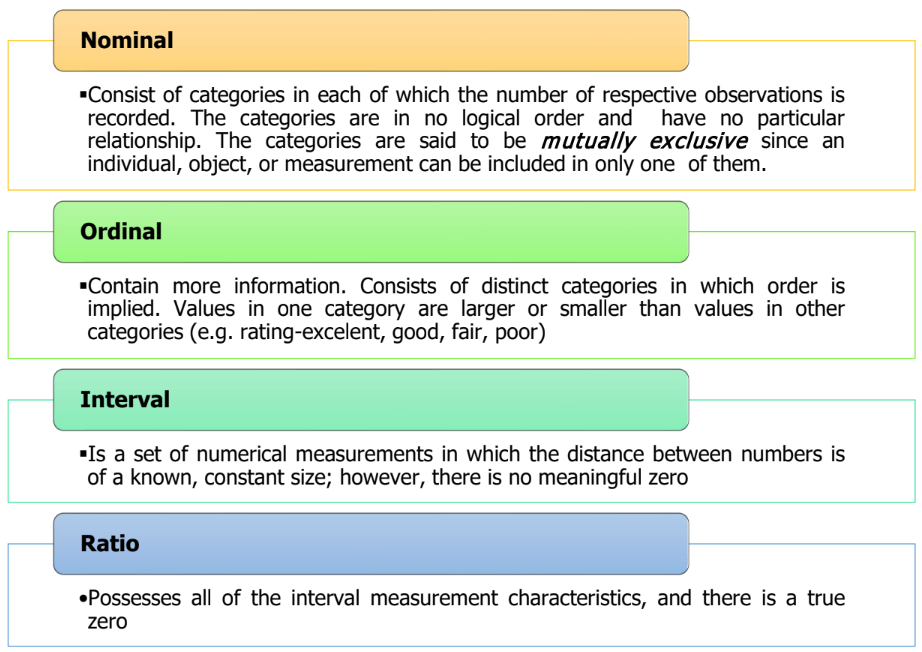
\includegraphics[width=5.20833in,height=\textheight]{images/ch1/Picture8.png}

{\textbf{Example 1.6}}

State the level of measurement for each variable below:

\begin{enumerate}
\def\labelenumi{\alph{enumi})}
\tightlist
\item
  The number of students in KAM2283A
\item
  Temperature in Malaysia
\item
  Stress level (Mild, Medium, Severe, Very Severe)
\item
  Food preference
\end{enumerate}

{\textbf{Answer}}

\begin{enumerate}
\def\labelenumi{\alph{enumi})}
\tightlist
\item
  Ratio
\item
  Interval
\item
  Ordinal
\item
  Nominal
\end{enumerate}

\hypertarget{sampling}{%
\section{Sampling}\label{sampling}}

Sampling is a process of taking a subset of element from a population.
The sample taken from the sampling process have a same characteristic
with its population. However, the samples selected are not a perfect
representative of population depending on where they are selected.
Therefore, there always occur some error in the result of analysis
called as sampling error. A \textbf{sampling error} is the difference
between the results obtained from a sample and the results obtained from
the population.

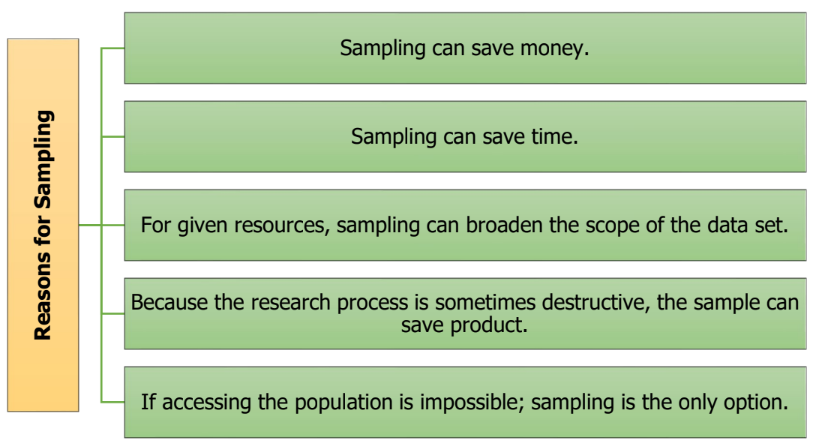
\includegraphics[width=5.20833in,height=\textheight]{images/ch1/Picture9.png}

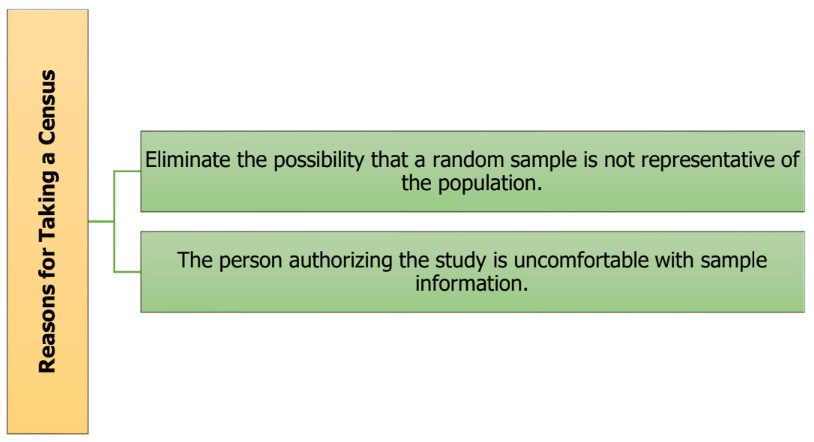
\includegraphics[width=5.20833in,height=\textheight]{images/ch1/Picture10.png}

\hypertarget{sampling-method}{%
\section{Sampling Method}\label{sampling-method}}

Random vs Non-Random sampling

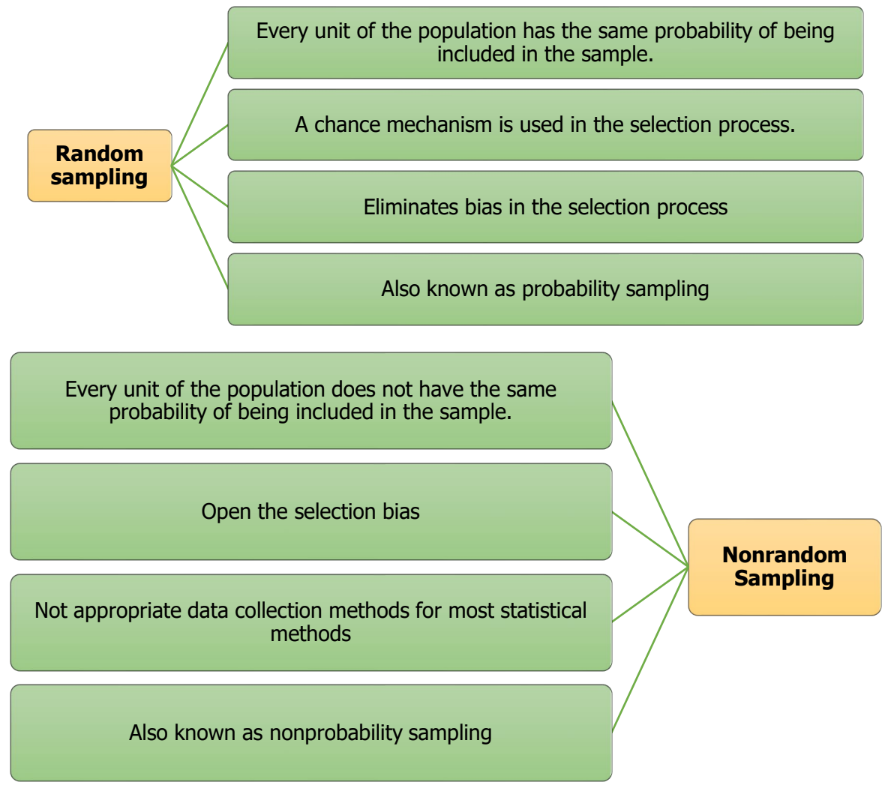
\includegraphics[width=5.20833in,height=\textheight]{images/ch1/Picture11.png}

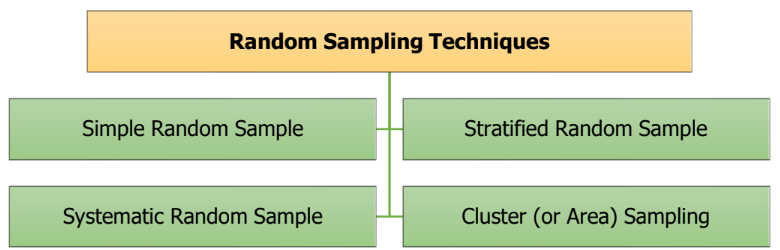
\includegraphics[width=5.20833in,height=\textheight]{images/ch1/Picture12.png}

\hypertarget{simple-random-sample}{%
\subsection{Simple Random Sample}\label{simple-random-sample}}

\begin{itemize}
\tightlist
\item
  Number each frame unit from 1 to N.
\item
  Use a random number table or a random number generator to select n
  distinct numbers between 1 and N, inclusively.
\item
  Easier to perform for small populations.
\item
  Cumbersome for large populations
\end{itemize}

\begin{figure}

{\centering 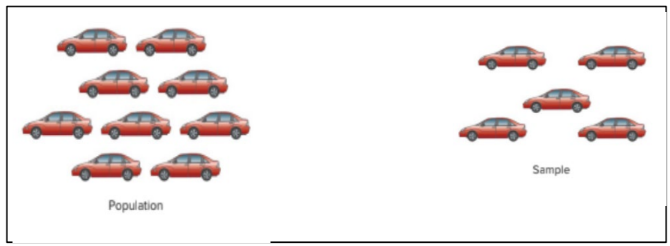
\includegraphics[width=5.20833in,height=\textheight]{images/ch1/Picture13.png}

}

\caption{Source: Allan G. Bluman (2010)}

\end{figure}

\hypertarget{systematic-sampling}{%
\subsection{Systematic Sampling}\label{systematic-sampling}}

\begin{itemize}
\tightlist
\item
  Convenient and relatively easy to administer.
\item
  Population elements are an ordered sequence (at least, conceptually).
\item
  The first sample element is selected randomly from the first k
  population elements.
\item
  Thereafter, sample elements are selected at a constant interval, k,
  from the ordered sequence frame.
\end{itemize}

\begin{figure}

{\centering 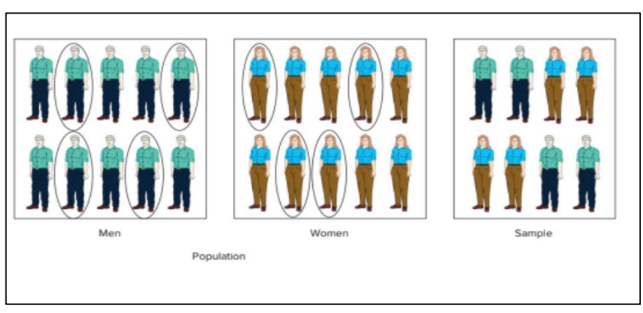
\includegraphics[width=5.20833in,height=\textheight]{images/ch1/Picture14.png}

}

\caption{Source: Allan G. Bluman (2010)}

\end{figure}

\hypertarget{stratified-random-sample}{%
\subsection{Stratified Random Sample}\label{stratified-random-sample}}

\begin{itemize}
\tightlist
\item
  Population is divided into nonoverlapping subpopulations called
  strata.
\item
  A random sample is selected from each stratum.
\item
  Potential for reducing sampling error.
\item
  Proportionate -- the percentage of the sample taken from each stratum
  is proportionate to the percentage that each stratum is within the
  population.
\item
  Disproportionate -- proportions of the strata within the sample are
  different than the proportions of the strata within the population.
\end{itemize}

\begin{figure}

{\centering 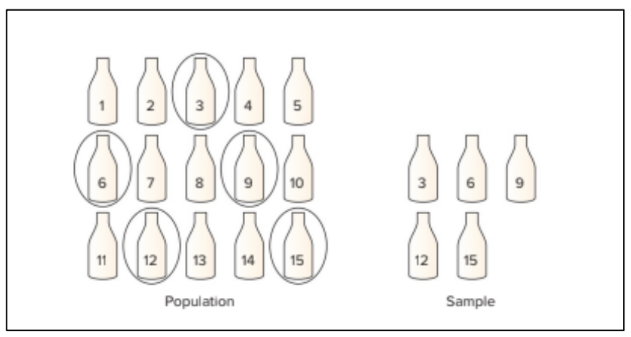
\includegraphics[width=5.20833in,height=\textheight]{images/ch1/Picture15.png}

}

\caption{Source: Allan G. Bluman (2010)}

\end{figure}

\hypertarget{cluster-sampling}{%
\subsection{Cluster Sampling}\label{cluster-sampling}}

\begin{itemize}
\tightlist
\item
  Population is divided into non overlapping clusters or areas
\item
  Each cluster is a miniature, or microcosm, of the population.
\item
  A subset of the clusters is selected randomly for the sample.
\item
  If the number of elements in the subset of clusters is larger than the
  desired value of n, these clusters may be subdivided to form a new set
  of clusters and subjected
\end{itemize}

\begin{figure}

{\centering 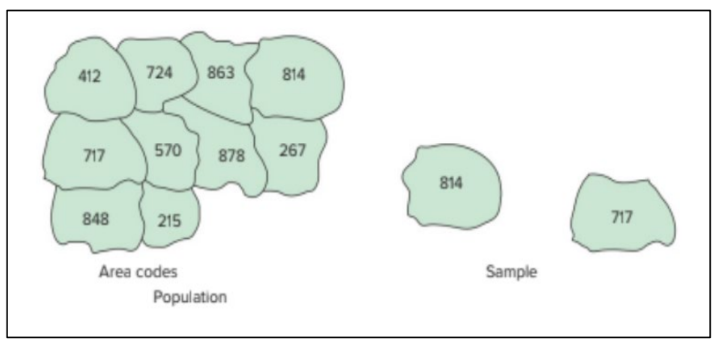
\includegraphics[width=5.20833in,height=\textheight]{images/ch1/Picture16.png}

}

\caption{Source: Allan G. Bluman (2010)}

\end{figure}

\textbf{Advantages}

\begin{itemize}
\tightlist
\item
  More convenient for geographically dispersed populations.
\item
  Reduced travel costs to contact sample elements.
\item
  Simplified administration of the survey.
\item
  Unavailability of sampling frame prohibits using other random sampling
  methods.
\end{itemize}

\textbf{Disadvantages}

\begin{itemize}
\tightlist
\item
  Statistically less efficient when the cluster elements are similar.
\item
  Costs and problems of statistical analysis are greater than for simple
  random sampling to a random selection process.
\end{itemize}

\hypertarget{nonrandom-sampling}{%
\subsection{Nonrandom Sampling}\label{nonrandom-sampling}}

\begin{enumerate}
\def\labelenumi{\arabic{enumi}.}
\tightlist
\item
  \textbf{Convenience Sampling}: sample elements are selected for the
  convenience of the researcher.
\item
  \textbf{Judgement Sampling}: sample elements are selected by the
  judgment of the researcher.
\item
  \textbf{Quota Sampling}: sample elements are selected until the quota
  controls are satisfied.
\item
  \textbf{Snowball Sampling}: survey subjects are selected based on a
  referral from other survey respondents
\end{enumerate}

\hypertarget{exercise-1}{%
\section{Exercise 1}\label{exercise-1}}

\begin{enumerate}
\def\labelenumi{\arabic{enumi}.}
\tightlist
\item
  A private company manager is interested in studying the relationship
  between time spent on social media and employee performance. He
  believed that the more time spent on social media, the more likely the
  performance drops. The performance of the employee is categorized as
  excellent, moderate, and low. A random sample of 500 employees was
  selected for this study, and the time spent on social media was
  recorded.
\end{enumerate}

\begin{enumerate}
\def\labelenumi{\alph{enumi})}
\tightlist
\item
  State the population and the sample for the above study.
\item
  Identify whether the study was conducted by a census or sample survey.
  Give a reason.
\item
  Identify the variable of this study.
\end{enumerate}

\begin{enumerate}
\def\labelenumi{\arabic{enumi}.}
\setcounter{enumi}{1}
\tightlist
\item
  A lecturer from a private college wanted to estimate how much their
  students spent (in RM) on reference books for a semester. From a total
  of 300 students, only 12 students randomly selected as a sample. The
  distribution of the number of students is shown in the following
  table.
\end{enumerate}

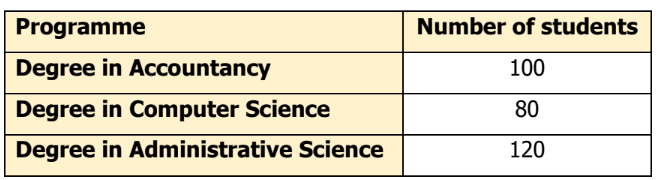
\includegraphics[width=5.20833in,height=\textheight]{images/ch1/Picture17.png}

\begin{enumerate}
\def\labelenumi{\alph{enumi})}
\tightlist
\item
  State the population and sample.
\item
  State the variable of the study.
\end{enumerate}

\begin{enumerate}
\def\labelenumi{\arabic{enumi}.}
\setcounter{enumi}{2}
\tightlist
\item
  A registrar in University F would like to study the readiness of
  students returning to campus after one year staying at home learning
  through online platform. For this purpose, students are listed
  according to their student ID. An online questionnaire was distributed
  randomly to 1000 students. The readiness is scale from 1 (Strongly not
  ready) to 10 (Strongly ready).
\end{enumerate}

\begin{enumerate}
\def\labelenumi{\alph{enumi})}
\tightlist
\item
  State the population, sample and sampling frame.
\item
  Identify the variable of interest.
\end{enumerate}

\begin{enumerate}
\def\labelenumi{\arabic{enumi}.}
\setcounter{enumi}{3}
\tightlist
\item
  Determine whether \textbf{Descriptive Statistics} or
  \textbf{Inferential Statistics} were used.
\end{enumerate}

\begin{enumerate}
\def\labelenumi{\alph{enumi})}
\tightlist
\item
  Based on the bar chart, the highest sales for Company XYZ are on
  December.
\item
  There is an association between gender and level of stress.
\item
  A scientist found that a good laugh significantly reduces person's
  stress level.
\item
  The distribution number of male patients received a treatment in
  Hospital Y is skewed to the right.
\item
  Sales for Company Y are more consistent than Company X.
\item
  Based on a sample of 300 students, the dean has enough evidence to
  conclude that students more prefer face-to-face classes compared to
  online classes.
\item
  A study conducted by a research network found that people with fewer
  than 12 years of education had lower life expectancy than those with
  more years of education.
\item
  In 2025, the Save Hypermarket is predicted their sales to be RM 5.3
  billion.
\end{enumerate}

\begin{enumerate}
\def\labelenumi{\arabic{enumi}.}
\setcounter{enumi}{4}
\tightlist
\item
  Decide whether it is primary data or secondary data.
\end{enumerate}

\begin{enumerate}
\def\labelenumi{\alph{enumi})}
\tightlist
\item
  Personal Interview.
\item
  Data from Statistical Department.
\item
  A study is undertaken to find the labour productivity of Hypermarket
  Berjaya at two locations. For this purpose, selected laborers in both
  locations is contacted and their productivity figures are noted.
\item
  Data obtained from the Kaggle website is being used by students for
  research courses.
\item
  Data collected by the Ministry of Health are being used by the
  scientist, academicians and etc for their further study.
\end{enumerate}

\begin{enumerate}
\def\labelenumi{\arabic{enumi}.}
\setcounter{enumi}{5}
\tightlist
\item
  State whether the following quantitative (discrete or continuous) or
  qualitative variable.
\end{enumerate}

\begin{enumerate}
\def\labelenumi{\alph{enumi})}
\tightlist
\item
  Distance
\item
  Litres of petrol
\item
  Level of anxiety
\item
  Depression score
\item
  Sizes of drinks sold by restaurant (small, medium and large)
\item
  Number of patients waiting for treatment
\item
  Length of time
\item
  Temperature at a Hawaii Resort
\item
  Rating of lecturer
\end{enumerate}

\begin{enumerate}
\def\labelenumi{\arabic{enumi}.}
\setcounter{enumi}{6}
\tightlist
\item
  State the level of measurement for the following variable.
\end{enumerate}

\begin{enumerate}
\def\labelenumi{\alph{enumi})}
\tightlist
\item
  Size of blouse (36,38,40,42)
\item
  The height of building
\item
  The number accident case .
\item
  Stress level (Mild, Medium, Severe, Very Severe)
\item
  Satisfaction level (1(very unsatisfied) to 5(very satisfied)
\end{enumerate}

\begin{enumerate}
\def\labelenumi{\arabic{enumi}.}
\setcounter{enumi}{7}
\tightlist
\item
  What types of sampling technique used for each situation?
\end{enumerate}

\begin{enumerate}
\def\labelenumi{\alph{enumi})}
\tightlist
\item
  A lecturer conducts a study to collect data on students' performance
  in the Statistics course. The lecturer randomly selects five classes
  from ten and samples all students in those five classes.
\item
  Newton Car operates ten dealerships in ten states, including Sabah and
  Sarawak. The Head of Service Department is interested to know about
  the car problems encountered by their customers. Only 150 customers
  are chosen as respondents for each branch.
\item
  The manager of Hotel Hibiscus instructed an HR Department to ask about
  customer satisfaction after a stay at their hotel. The customers are
  selected randomly.
\item
  The number of students passed in probability subject decreasing every
  semester. A lecturer is concerned with the issue and wants to know the
  problem and identify the issue. From 50 students, only 10 students
  with weak academic records are chosen.
\item
  In order to choose a suitable platform for an online class, students
  were asking for their opinion.
\end{enumerate}

\begin{enumerate}
\def\labelenumi{\arabic{enumi}.}
\setcounter{enumi}{8}
\tightlist
\item
  State the best sampling method that can be used for the study below:
\end{enumerate}

\begin{enumerate}
\def\labelenumi{\alph{enumi})}
\tightlist
\item
  A group of researchers conducted a study on the satisfaction of
  parents with online learning classes for primary school in Kedah. For
  that purpose, the researchers set out to conduct a survey and limit a
  selection of sample, 100 parents from rural areas and 200 parents from
  urban area.
\item
  The audit team selects every 20th box out of a total of 100 boxes to
  test the quality of Product X. All of the product X in the selected
  box is sampled in order to assess the product's defects.
\end{enumerate}

\hypertarget{turorial-1}{%
\section{Turorial 1}\label{turorial-1}}

\textbf{Question 1}

A group of researchers wanted to investigate the perception of the
married couple towards on the factors that contributed to the marriage
problems in Perak. The researchers distributed the questionnaires to 500
randomly selected couples from four districts (I, II, III, IV) in the
state. Twenty-five items on the perception towards on the factors
contributed to the marriage problems were measured using Likert Scale
(strongly agree=1, agree=2, neutral=3, disagree=4, strongly disagree=5).
The distribution on the number of married couples is shownin the
following table.

\begin{longtable}[]{@{}cc@{}}
\toprule\noalign{}
District & Number of married couples \\
\midrule\noalign{}
\endhead
\bottomrule\noalign{}
\endlastfoot
I & 500 \\
II & 450 \\
III & 300 \\
IV & 350 \\
\end{longtable}

\begin{enumerate}
\def\labelenumi{\alph{enumi})}
\tightlist
\item
  State the population of the above study.
\item
  State the sampling frame for the above study.
\item
  State the variable involve for this study. Hence, identify the
  corresponding scales of measurements.
\item
  Name the sampling method used in this study. Explain your answer in
  the context of the study.
\end{enumerate}

\textbf{Question 2}

In the automobile industry, customer service is a crucial factor
affecting car sales. The management of a reputed automobile company is
interested in determining the level of customers' satisfaction with the
service provided by the company's service centres. The company has
altogether 40 service centres throughout Malaysia. A sample of eight
centres was selected at random. Questionnaires are disseminated to all
customers who service their cars at these eight selected services
centres on one selected day (the day of the survey). One of the
questions asked is satisfaction level on the services provided (using
rating: good, fair, poor)

\begin{enumerate}
\def\labelenumi{\alph{enumi})}
\tightlist
\item
  State the population of the study.
\item
  Name the variable of interest for the above study. State its type and
  level of measurement.
\item
  Identify the sampling technique used. Explain briefly how the sample
  is selected.
\end{enumerate}

\textbf{Question 3}

A researcher wishes to study students' satisfaction (strongly
disagree=l, disagree=2, neutral=3, agree=4, strongly agree=5) towards
the services provided by the Academic Affairs in Nursing College X. The
researcher chooses only 10 out of 50 classes. All the students from
these 10 classes will be used for the study.

\begin{enumerate}
\def\labelenumi{\alph{enumi})}
\tightlist
\item
  Identify the population for the above study.
\item
  State the sampling frame for the above study.
\item
  Name the variable of interest for the above study. State its type and
  its level of measurement.
\item
  State the sampling technique used in this study.
\end{enumerate}

\textbf{Question 4}

A researcher is interested in studying the career aspirations of
students from the Faculty of Electrical Engineering, which consists of
30 classes. The researcher intends to choose all the students from 5
classes for the study.

\begin{enumerate}
\def\labelenumi{\alph{enumi})}
\tightlist
\item
  State the population and the sample for the above study.
\item
  Identify the variable of interest for this study and state the type of
  variable used.
\item
  What is the sampling technique used in this study?
\item
  Name ONE (1) method of data collection suitable for this study? Give
  ONE (1) advantage of using this method.
\end{enumerate}

\textbf{Question 5}

A survey on the workers' satisfaction levels was carried out at Company
XY. The company has 24 branches with the same setting. A sample of 6
branches was selected at random. All workers who work at these 6
branches were then selected for the study.

\begin{enumerate}
\def\labelenumi{\alph{enumi})}
\tightlist
\item
  State the population of the study.
\item
  State the sampling frame for the survey.
\item
  State the variable for this study. What type of variable is it?
\item
  Name the sampling technique used in the study.
\item
  Besides the sampling technique used in (d), briefly explain how the
  sample of 6 branches can be selected using systematic sampling
  technique.
\item
  What is the most suitable data collection method to be used for the
  study? Give one advantage of the suggested method.
\end{enumerate}

\textbf{Question 6}

Employers were surveyed to determine the level of satisfaction with
their employees who are graduated from ICT courses at University YY.
This study involved 50 employers from ICT private companies from five
randomly chosen states out of 14. All selected employers were asked
about gender, length of service (years), how well graduates meet
employer expectations (1=Excellent, 2=Average, and 3=Poor), and overall
employer's satisfaction with graduates (1=Excellent, 2=Average, and
3=Poor).

\begin{enumerate}
\def\labelenumi{\alph{enumi})}
\tightlist
\item
  State the population and sampling frame.
\item
  Name any TWO (2) variables from the study. Hence, state its type of
  variable.
\item
  Name the sampling technique employed in the study.
\item
  Suggest the data collection method that suitable to the study. Give
  ONE (1) advantage of the method used.
\end{enumerate}

\textbf{Question 7}

A manager at one of the popular Telco company is currently conducting a
survey regarding the service failure at their service counter. The main
objective of the survey is to find out the factors that cause the
failure. He randomly selected five service counters from ten available
service counters all over Malaysia. A questionnaire is distributed to
all the customers at the five selected service counters. The information
collected from the customers include age, gender, occupation, income,
rating of service (0 to 100) and service quality (poor, moderate and
good).

\begin{enumerate}
\def\labelenumi{\alph{enumi})}
\item
  State the population in the study.
\item
  State the sampling technique used in the study.
\item
  Identify one ordinal variable and one ratio variable obtained from the
  study.
\item
  The followings are the statistics produced from the study. Identify
  whether each statement is a descriptive or inferential statistics.

  \begin{enumerate}
  \def\labelenumii{\roman{enumii})}
  \tightlist
  \item
    45\% of the sample customers work in the government sector.
  \item
    Based on the sample, it can be concluded that there is an
    association between gender and service quality.
  \item
    We are 90\% confident that the average rating of service of for the
    customers falls between 60 and 90.
  \end{enumerate}
\end{enumerate}

\hypertarget{answer-to-tutorial-1}{%
\section{Answer to Tutorial 1}\label{answer-to-tutorial-1}}

\textbf{Question 1}

\begin{enumerate}
\def\labelenumi{\alph{enumi})}
\tightlist
\item
  All married couples in Perak.
\item
  List of all married couples from four districts in Perak.
\item
  Perception; Nominal.
\item
  Stratified Sampling Technique. Determine the number of samples from
  each districts :
\end{enumerate}

\begin{longtable}[]{@{}ccc@{}}
\toprule\noalign{}
District & Number of married couples & Number of samples \\
\midrule\noalign{}
\endhead
\bottomrule\noalign{}
\endlastfoot
I & 500 & (500/1600)*500=156 \\
II & 450 & 141 \\
III & 300 & 94 \\
IV & 350 & 109 \\
& & 500 \\
\end{longtable}

\textbf{Question 2}

\begin{enumerate}
\def\labelenumi{\alph{enumi})}
\tightlist
\item
  All customers at all 40 services centre in Malaysia.
\item
  Customer satisfaction; qualitative; ordinal
\item
  Cluster sampling technique.
\end{enumerate}

\textbf{Question 3}

\begin{enumerate}
\def\labelenumi{\alph{enumi})}
\tightlist
\item
  All students at Nursing College X.
\item
  List of all students from ten classes.
\item
  Students' satisfaction; qualitative ; ordinal
\item
  Cluster sampling technique.
\end{enumerate}

\textbf{Question 4}

\begin{enumerate}
\def\labelenumi{\alph{enumi})}
\tightlist
\item
  Population : All students from Faculty of Electrical Engineering.
  Sample: All students from five classes.
\item
  Career aspiration; qualitative; nominal
\item
  Cluster sampling technique
\item
  Self-administrative questionnaire. Advantage: quick response
\end{enumerate}

\textbf{Question 5}

\begin{enumerate}
\def\labelenumi{\alph{enumi})}
\tightlist
\item
  All workers at Company XY.
\item
  List of all workers at six branches at Company XY.
\item
  Satisfaction; qualitative
\item
  Cluster sampling technique.
\item
  N=24, n =6; k= 24/6 = 4; in first interval choose any number from 1
  until 4. let say, choose number 2. The number 2 will be the first
  sample. Next interval from 5 until 8. Continue select the samples
  until you reach 6 samples.
\item
  Email questionnaires.
\end{enumerate}

\textbf{Question 6}

\begin{enumerate}
\def\labelenumi{\alph{enumi})}
\setcounter{enumi}{4}
\tightlist
\item
  Population: All employers in the ICT private companies who are
  employed ICT graduates from University YY. Sampling frame: A list name
  of ICT company who are employed ICT graduated from University YY.
\item
  Gender (Qualitative); length of services (Quantitative Continuous),
  employer's expectations (Qualitative), and employer's satisfaction
  with graduates (Qualitative).
\item
  Cluster sampling
\item
  Internet survey (Google form)/ Electronic questionnaire. Fast and
  short in time span to complete the questionnaire, cheaper. Any
  relevant answer.
\end{enumerate}

\textbf{Question 7}

\begin{enumerate}
\def\labelenumi{\alph{enumi})}
\item
  Population: All customers from 10 service counters all over Malayisa
\item
  Cluster sampling
\item
  Ordinal variable : service quality; ratio variable : age/ income
\item
  \begin{enumerate}
  \def\labelenumii{\roman{enumii})}
  \tightlist
  \item
    Descriptive, ii) Inferential iii) Inferential
  \end{enumerate}
\end{enumerate}

\bookmarksetup{startatroot}

\hypertarget{descriptive-statistics}{%
\chapter{Descriptive Statistics}\label{descriptive-statistics}}

\hypertarget{learning-objectives-1}{%
\section*{Learning objectives:}\label{learning-objectives-1}}
\addcontentsline{toc}{section}{Learning objectives:}

\markright{Learning objectives:}

\begin{enumerate}
\def\labelenumi{\arabic{enumi}.}
\tightlist
\item
  Identify various ways to present collected data from survey of
  secondary sources
\item
  Use appropriate data presentation for a qualitative and quantitative
  data
\item
  Calculate the measures of central tendency, measure of variation,
  measure of skewness and measure of position for ungrouped data.
\end{enumerate}

\hypertarget{introduction-1}{%
\section{Introduction}\label{introduction-1}}

When conducting a statistical study, the researcher must gather data for
the variable under study. For example, if a researcher wishes to study
the number of road accidents in Malaysia for the past 2 years, he or she
must gather the data from various departments. To describe the
situation, draw conclusions, or make inferences about the event, the
researcher must organize the data and present it in some meaningful way.

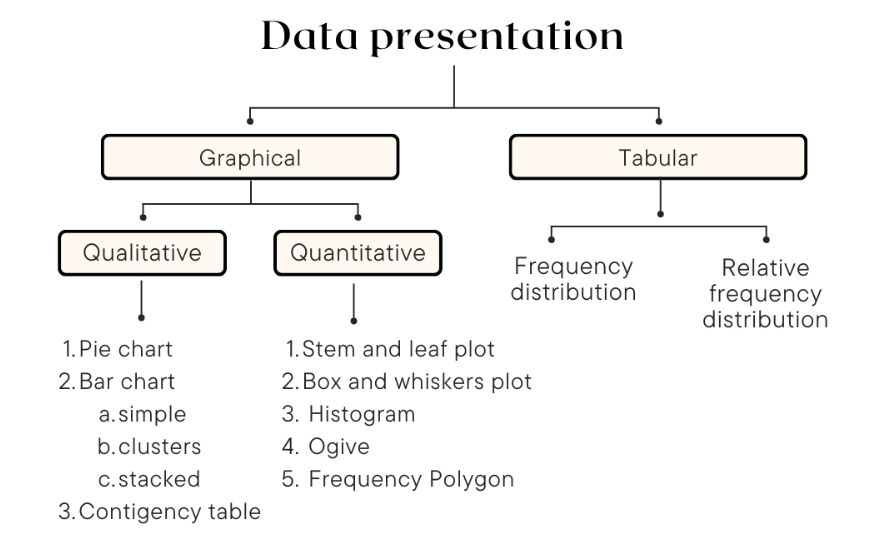
\includegraphics[width=6.25in,height=\textheight]{images/ch2/picture1.png}

The data can be presented in term of graphical approach or table and
numerical descriptive measure for both qualitative dan quantitative
data.

\hypertarget{organizing-data}{%
\section{Organizing Data}\label{organizing-data}}

\textbf{Charts and graphs}

\begin{itemize}
\tightlist
\item
  Frequency distributions are good ways to present the essential aspects
  of data collections in concise and understandable terms
\item
  Pictures are always more effective in displaying large data
  collections
\end{itemize}

\textbf{Histogram}

\begin{itemize}
\tightlist
\item
  Frequently used to graphically present interval and ratio data
\item
  The adjacent bars indicate that a numerical range is being summarized
  by indicating the frequencies in arbitrarily chosen classes
\end{itemize}

\begin{figure}

{\centering 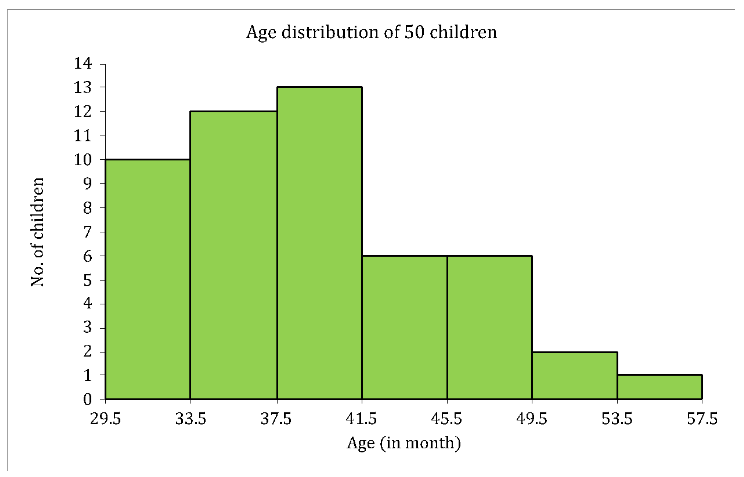
\includegraphics[width=5.20833in,height=\textheight]{images/ch2/picture2.png}

}

\caption{Figure 1: Histogram -- distribution of the ages (in months) of
50 children}

\end{figure}

\textbf{Frequency Polygon}

\begin{itemize}
\tightlist
\item
  Another common method for graphically presenting interval and ratio
  data
\item
  To construct a frequency polygon mark the frequencies on the vertical
  axis and the values of the variable being measured on the horizontal
  axis, as with the histogram.
\item
  If the purpose of presenting is to compare with other distributions,
  the frequency polygon provides a good summary of the data
\end{itemize}

\begin{figure}

{\centering 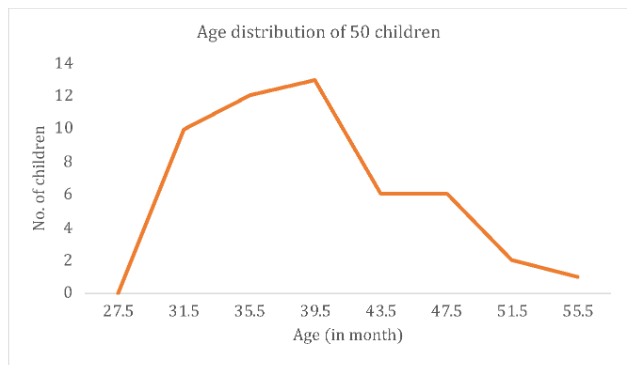
\includegraphics[width=5.20833in,height=\textheight]{images/ch2/picture3.png}

}

\caption{Figure 2: Frequency Polygon -- distribution of the ages (in
months) of 50 children}

\end{figure}

\textbf{Ogive}

\begin{itemize}
\tightlist
\item
  A graph of a cumulative frequency distribution
\item
  Ogive is used when one wants to determine how many observations lie
  above or below a certain value in a distribution.
\item
  First cumulative frequency distribution is constructed
\item
  Cumulative frequencies are plotted at the upper-class limit of each
  category
\item
  Ogive can also be constructed for a relative frequency distribution.
\end{itemize}

\begin{figure}

{\centering 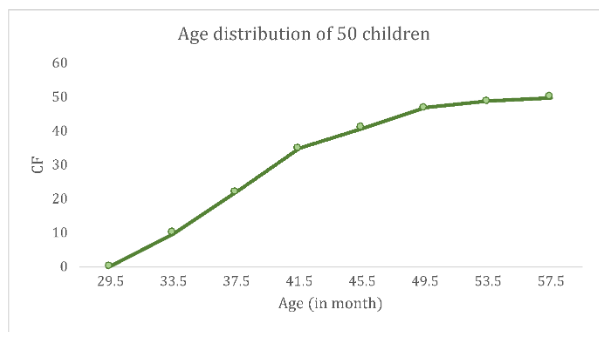
\includegraphics[width=5.20833in,height=\textheight]{images/ch2/picture4.png}

}

\caption{Figure 3: Ogive distribution of the ages (in months) of 50
children}

\end{figure}

\textbf{Pie Chart}

\begin{itemize}
\tightlist
\item
  The pie chart is an effective way of displaying the percentage
  breakdown of data by category.
\item
  The size of angle (°) is determined based on the frequency of
  group/category
\item
  Useful if the relative sizes of the data components are to be
  emphasized Pie charts also provide an effective way of presenting
  ratio- or interval-scaled data after they have been organized into
  categories
\item
  How to compute angle/degree? \[
  x^{\circ} = \frac{f}{\sum{x}} \times 360
  \]
  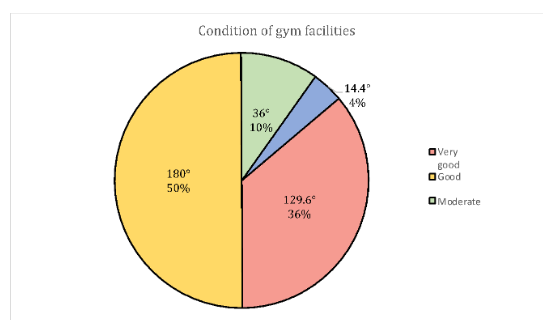
\includegraphics[width=5.20833in,height=\textheight]{images/ch2/picture5.png}
\end{itemize}

\textbf{Bar Charts}

\begin{itemize}
\tightlist
\item
  Another common method for graphically presenting nominal and ordinal
  scaled data
\item
  One bar is used to represent the frequency for each category
\item
  The bars are usually positioned vertically with their bases located on
  the horizontal axis of the graph
\item
  The bars are separated, and this is why such a graph is frequently
  used for nominal and ordinal data -- the separation emphasize the
  plotting of frequencies for distinct categories
\end{itemize}

\begin{figure}

{\centering 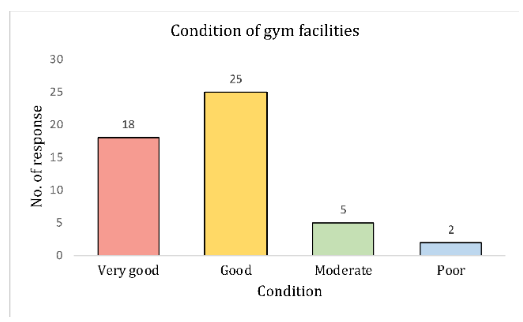
\includegraphics[width=5.20833in,height=\textheight]{images/ch2/picture6.png}

}

\caption{Figure 5: Bar Chart -- Condition of gym facilities}

\end{figure}

\textbf{Stem and Leaf}

A \emph{stem and leaf plot} is a data plot that uses part of a data
value as the stem and part of the data value as the leaf to form groups
or classes.

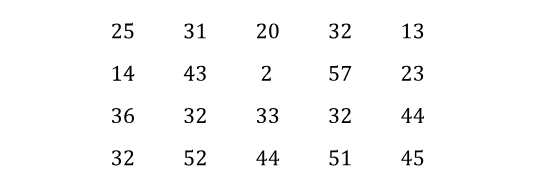
\includegraphics[width=5.20833in,height=\textheight]{images/ch2/picture7.png}

\begin{figure}

{\centering 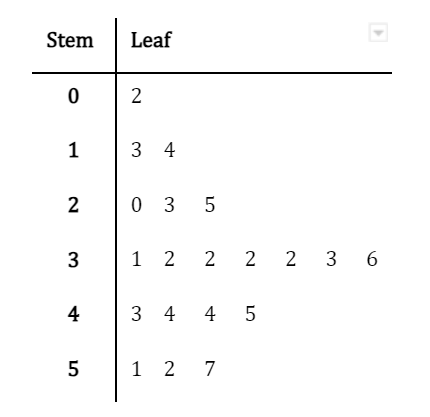
\includegraphics[width=5.20833in,height=\textheight]{images/ch2/picture8.png}

}

\caption{Figure 6: Stem-and-Leaf Diagram}

\end{figure}

\hypertarget{numerical-descriptive-measures-ungrouped}{%
\section{Numerical descriptive measures
(ungrouped)}\label{numerical-descriptive-measures-ungrouped}}

\begin{itemize}
\tightlist
\item
  Measures of central tendency (mean, median, mode)
\item
  Measure of variation (range, standard deviation, variance, coefficient
  of variation
\item
  Measure of skewness
\item
  Measures of Position (Q1, Q2, and Q3)
\end{itemize}

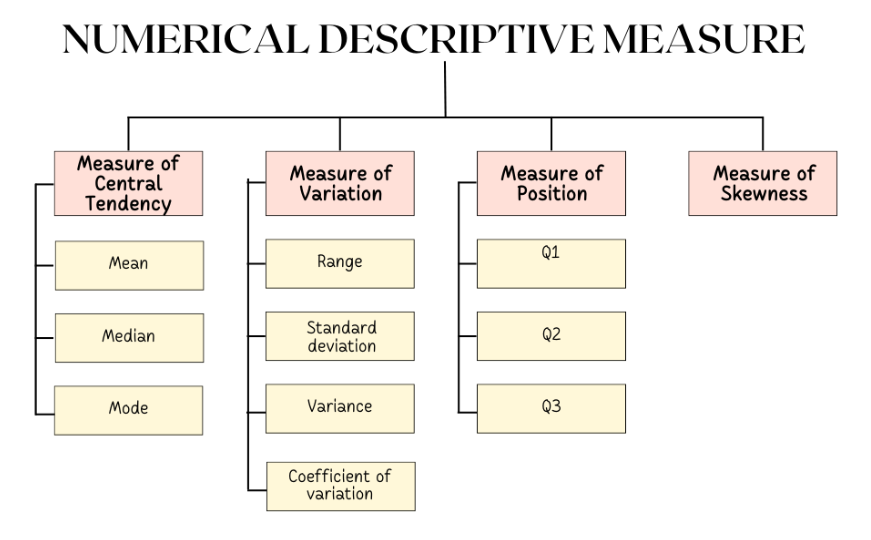
\includegraphics[width=6.25in,height=\textheight]{images/ch2/picture9.png}

\hypertarget{measures-of-central-tendency}{%
\subsection{Measures of Central
Tendency}\label{measures-of-central-tendency}}

\textbf{Mean}

The mean is the quotient of the sum of the values and the total number
of values. The symbol \(\bar{x}\) is used for \textbf{sample mean} and
is given by the following formula:

\[
\bar{x} = \frac{x_1 + x_2 + x_3 + ... + x_{n-1} + x_n}{n} = \frac{\sum{x}}{n}
\] For a population, the Greek letter \(\mu\) (mu) is used for the mean.

\[
\bar{X} = \frac{X_1 + X_2 + X_3 + ... + X_{n-1} + X_N}{N} = \frac{\sum{X}}{N}
\]

{\textbf{Example 2.1}}

The number of calls that a local police department responded to for a
sample of 9 months is shown. Find the mean.

475, 447, 440, 761, 993, 1052, 783, 671, 621

{\textbf{Answer}}

\[
\begin{aligned}
\bar{x} = \frac{\sum{x}}{n} &= \frac{475+447+440+761+993+1052+783+671+621}{9} \\
&= \frac{6243}{9} \approx 693.7
\end{aligned}
\]

\textbf{Interpretation:} On average, the number of calls responded by
local police department is approximately 694 calls.

{\textbf{Example 2.2}}

A climatologist recorded daily temperature in Sungai Petani for twelve
days. The data points are as follows (in degrees Celsius):

30.5, 31.2, 29.8, 30.0, 30.7, 31.5, 29.9, 30.3, 30.1, 31.0, 30.4, 31.8

Calculate the mean of daily temperature, and interpretation of the
meaning of the mean value.

{\textbf{Answer}}

\[
\begin{aligned}
\bar{x} &= \frac{30.5+31.2+29.8+30.0+30.7+31.5+29.9+30.3+30.1+31.0+30.4+31.8}{12} \\
&= 30.75^\circ C
\end{aligned}
\] On average, the daily temperatures in Sungai Petani for twelve days
is \(30.75^\circ C\).

{\textbf{Example 2.3}}

In a bakery, the number of doughnuts sold in 7 days is recorded as
follows:

53, 60, 45, 77, 58, 42, 68

{\textbf{Answer}}

\[
\begin{aligned}
\bar{x} &= \frac{53 + 60 + 45 + 77 + 58 + 42 + 68}{7} \\
&= 57.57
\end{aligned}
\]

On average, the number of doughnuts sold in seven days is approximately
58 doughnuts.

\textbf{Properties of the Mean}

\begin{itemize}
\tightlist
\item
  Found by using all the values of data.
\item
  Varies less than the median or mode.
\item
  Used in computing other statistics, such as the variance.
\item
  Unique, usually not one of the data values.
\item
  Cannot be used with open-ended classes.
\item
  Affected by extremely high or low values, called outliers.
\end{itemize}

\textbf{Median}

The \textbf{median} is the midpoint of the data array. The symbol for
the median is \(\tilde{x}\). How to identify median value?

\begin{enumerate}
\def\labelenumi{\roman{enumi}.}
\tightlist
\item
  Sort the data in ascending order
\item
  Identify the location of median using
\item
  Determine the value of median
\end{enumerate}

\begin{itemize}
\tightlist
\item
  If the number of data (n) is ODD, the value is in the middle of
  sequence
\item
  If the number of data (n) is EVEN, the value of median is average of 2
  middle values
\end{itemize}

{\textbf{Example 2.4}}

The number of police officers killed in the line of duty over the last
11 years is shown. Find the median.

175 152 121 142 188 154 160 165 148 156 239

{\textbf{Answer:}}

\begin{enumerate}
\def\labelenumi{\roman{enumi}.}
\tightlist
\item
  Sort the data in ascending order
\end{enumerate}

121, 142, 148, 152, 154, 156, 160, 165, 175, 188, 239

ii Identify the location of median:

\[
\frac{11 + 1}{2} = 6^{th}
\]

\begin{enumerate}
\def\labelenumi{\roman{enumi}.}
\setcounter{enumi}{2}
\tightlist
\item
  Select the middle value, \(\tilde{x} = 156\)
\end{enumerate}

{\textbf{Example 2.5}}

The number of tornadoes that have occurred in the certain country over
an 8-year period follows.

684, 764, 656, 702, 856, 1133, 1132, 1303

Find the median.

{\textbf{Answer:}}

Since the data given is even-number, there will be two values in the
middle.

\begin{enumerate}
\def\labelenumi{\roman{enumi}.}
\tightlist
\item
  Sort the data in ascending order
\end{enumerate}

656, 684, 702, 764, 856, 1132, 1133, 1303

ii Identify the location of median:

\[
\frac{8 + 1}{2} = 4.5^{th}
\]

\begin{enumerate}
\def\labelenumi{\roman{enumi}.}
\setcounter{enumi}{2}
\tightlist
\item
  Select the middle value,
  \(\tilde{x} = \frac{764 + 856}{2} = \frac{1620}{2} = 810\)
\end{enumerate}

\textbf{Interpretation of median:} Half of the tornadoes that have
occurred in a certain country is less than or equal to 810 of tornadoes.

\textbf{Properties of Median}

\begin{itemize}
\tightlist
\item
  Give the midpoint.
\item
  Used when it is necessary to find out whether the data values fall
  into the upper half or lower half of the distribution.
\item
  Can be used for an open-ended distribution.
\item
  Affected less than the mean by extremely high or extremely low values.
\end{itemize}

\textbf{Mode}

The \textbf{mode} is the value that occurs most often in a data set. It
is sometimes said to be the most typical case. There may be no mode, one
mode (unimodal), two modes (bimodal), or many modes (multimodal). Symbol
of the mode is \(\hat{x}\).

{\textbf{Example 2.6}}

Find the mode of the signing bonuses of eight football players for a
specific year. The bonuses in thousands of ringgit Malaysia (RM) are:

18.0, 14.0, 34.5, 10, 11.3, 10, 12.4, 10

{\textbf{Answer:}}

You may find it easier to sort first.

\textbf{10, 10, 10,} 11.3, 12.4, 14.0, 18.0, 34.5

Select the value that occurs the most.

\textbf{Interpretation:} Most of the players signed the bonuses of 10
thousand ringgits Malaysia.

{\textbf{Example 2.7}}

The data show the number of licensed nuclear reactors in the certain
country for a recent 15-year period. Find the mode.

103 103 103 103 103 106 108 108 108 110 108 112 112 112 108

{\textbf{Answer:}}

103 and 108 both occur the most. The data set is said to be bimodal. The
modals are 103 and 108.

\textbf{Properties of mode}

\begin{itemize}
\tightlist
\item
  Used when the most typical case is desired.
\item
  Easiest average to compute.
\item
  Can be used with nominal data.
\item
  Not always unique or may not exist.
\end{itemize}

\textbf{Distributions Shape}

\begin{figure}

{\centering 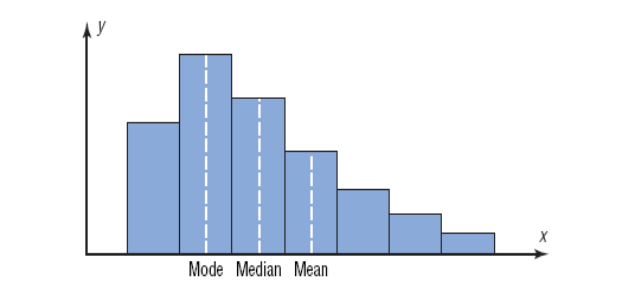
\includegraphics[width=5.20833in,height=\textheight]{images/ch2/picture10.png}

}

\caption{Figure 7: a) Positively skewed or right-skewed}

\end{figure}

\begin{figure}

{\centering 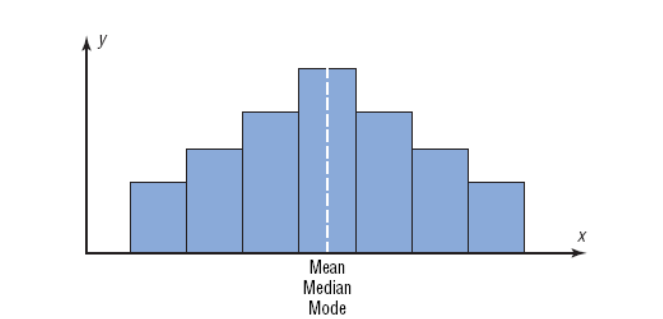
\includegraphics[width=5.20833in,height=\textheight]{images/ch2/picture11.png}

}

\caption{Figure 7: b) Symmetrical distribution since mean, mode and
median are equal}

\end{figure}

\begin{figure}

{\centering 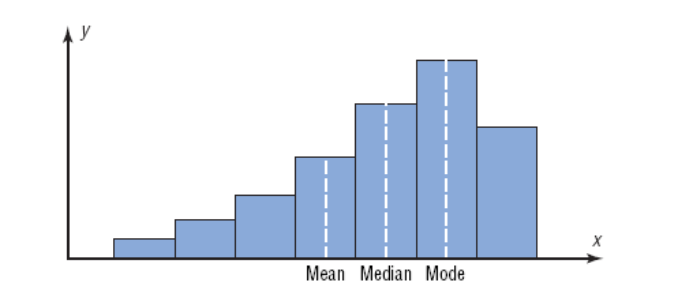
\includegraphics[width=5.20833in,height=\textheight]{images/ch2/picture12.png}

}

\caption{Figure 7: c) Negatively skewed or left-skewed}

\end{figure}

\hypertarget{measure-of-variation}{%
\subsection{Measure of variation}\label{measure-of-variation}}

Measures of variation include range, standard deviation, variance, and
coefficient of variation.

The \textbf{range} is the difference between the highest and lowest
values in a data set.

Range = Highest -- Lowest

The \textbf{population variance} is the average of the squares of the
distance each value is from the mean.

The \textbf{standard deviation} is the square root of the variance.

{\textbf{Example 2.8}}

The table below shows the life-long (in months) of two brands of paint.

\begin{longtable}[]{@{}cc@{}}
\toprule\noalign{}
Brand XX & Brand YY \\
\midrule\noalign{}
\endhead
\bottomrule\noalign{}
\endlastfoot
10 & 35 \\
60 & 45 \\
50 & 30 \\
30 & 35 \\
40 & 40 \\
20 & 25 \\
\end{longtable}

Determine the mean and standard deviation for the above data.

{\textbf{Answer:}}

{ Brand XX: \(\mu = mean = \frac{\sum{x}}{N} = \frac{210}{6} = 35\) and
\(Range = 60 - 10 = 50\). }

Brand YY: \(\mu = mean = \frac{\sum{x}}{N} = \frac{210}{6} = 35\) and
\(Range = 45 -25 = 20\).

The average for both brands is the same, but the range for Brand XX is
much greater than the range for Brand YY. Which brand would you buy?

\textbf{Uses of the Variance and Standard Deviation}

\begin{itemize}
\tightlist
\item
  To determine the spread of the data.
\item
  To determine the consistency of a variable.
\item
  To determine the number of data values that fall within a specified
  interval in a distribution (Chebyshev's Theorem).
\item
  Used in inferential statistics.
\end{itemize}

Population variance:

\[
\sigma^2 = \frac{\sum{(X - \mu)^2}}{N}
\]

Population Standard Deviation

\[
\sigma = \sqrt{ \frac{\sum{(X - \mu)^2}}{N}}
\]

Sample variance:

\[
s^2 = \frac{\sum{(X - \bar{X})^2}}{n-1}\ \ \ or\ \ \ s^2 = \frac{1}{n-1}\left[\sum{X^2} - \frac{(\sum{X})^2}{n}\right]
\]

Sample Standard Deviation:

\[
s = \sqrt{\frac{\sum{(X - \bar{X})^2}}{n-1}}\ \ \ or\ \ \ s = \sqrt{\frac{1}{n-1}\left[\sum{X^2} - \frac{(\sum{X})^2}{n}\right]}
\]

The \textbf{coefficient of variation} is the standard deviation divided
by the mean, expressed as a percentage.

\[
Coefficient\ of\ Variation\ (CV)\ = \frac{s}{x} \times 100\%
\]

{\textbf{Example 2.9}}

The mean of the number of sales of cars over a 3-month period is 87, and
the standard deviation is 5. The mean of the commissions is \$5225, and
the standard deviation is \$773. Compare the variations of the two.

{\textbf{Answer:}}

{\(CV_{Sales} = \frac{5}{87} \times 100\% = 5.7\%\)}

\(CV_{Commissions} = \frac{773}{5225} \times 100\% = 14.8\%\)

The data distribution for Commissions are more dispersed than sales.
Similarly, Sales data distribution is more consistent than the data
distribution in commissions.

{\textbf{Example 2.10}}

A meteorologist is studying the monthly rainfall patterns in two
different regions, Region A and Region B, over the past year. They have
collected data for 11 months (in mm). The goal is to determine which
region has more dispersed rainfall. Calculate the coefficient of
variation for each region's monthly rainfall data and identify which
region's data is more dispersed.

\begin{figure}

{\centering 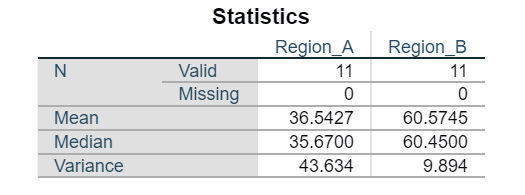
\includegraphics[width=4.16667in,height=\textheight]{images/ch2/picture13.png}

}

\caption{SPSS Output}

\end{figure}

{\textbf{Answer:}}

{\(CV_{Region A} = \frac{\sqrt{43.634}}{36.5427} \times 100\% = 18.08\%\)}

\(CV_{Region B} = \frac{\sqrt{9.894}}{60.5745} \times 100\% = 5.19\%\)

Region A has a more dispersed rainfall pattern than Region B.

\hypertarget{measure-of-skewness}{%
\subsection{Measure of skewness}\label{measure-of-skewness}}

Skewness is the measurement of the lack of symmetry of the distribution.
There are several measures for expressing the amount of skewness, but
the only important one is the Pearson Coefficient of Skewness:

\[
PCS = \frac{mean - mode}{standard\ deviation}\ \ \ \ or\ \ \ \ PCS = \frac{3(mean - median)}{standard\ deviation}
\]

\textbf{Skewness}

It is the \emph{degree of distortion} from the symmetrical bell curve or
the normal distribution. It measures the lack of symmetry in data
distribution. It differentiates extreme values in one versus the other
tail. A symmetrical distribution will have a skewness of 0.

There are two types of Skewness: \textbf{Positive} and
\textbf{Negative}.

\begin{figure}

{\centering 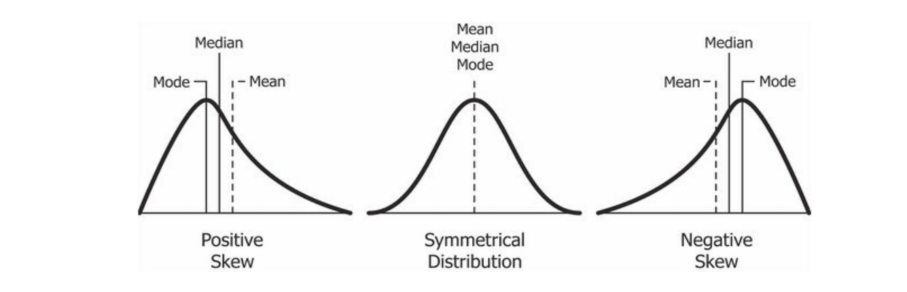
\includegraphics[width=5.20833in,height=\textheight]{images/ch2/picture14.png}

}

\caption{Figure 8: Types of Skewness}

\end{figure}

{\textbf{Example 2.11}}

The SPSS output gives information on descriptive statistics on the
number of licensed nuclear reactors in the certain country for a recent
15-year period. Find the Person Coefficient of Skewness. Hence identify
the shape of distribution.

{\textbf{Answer:}}

\begin{figure}

{\centering 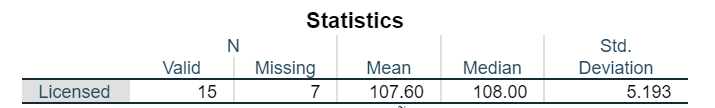
\includegraphics[width=4.16667in,height=\textheight]{images/ch2/picture15.png}

}

\caption{SPSS Output}

\end{figure}

\[
\begin{aligned}
PCS &= \frac{3(\bar{x} - \tilde{x})}{s} \\
&= \frac{3(107.6 - 108)}{5.193} \\
&= -0.2311
\end{aligned}
\]

Negatively skewed.

{\textbf{Example 2.12}}

The table below shows the number of eggs laid by 20 chickens over a
30-day period in a small poultry farm. Calculate the Pearson Coefficient
of Skewness. Hence identify the shape of distribution.

{\textbf{Answer:}}

\begin{figure}

{\centering 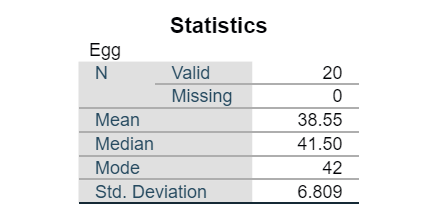
\includegraphics[width=4.16667in,height=\textheight]{images/ch2/picture16.png}

}

\caption{SPSS Output}

\end{figure}

\[
\begin{aligned}
PCS &= \frac{\bar{x} - \hat{x}}{s} \\
&= \frac{38.55 - 42}{6.809} \\
&= -0.5067
\end{aligned}
\]

Negatively skewed.

\hypertarget{measures-of-position-q-q2-and-q3}{%
\subsection{Measures of Position (Q, Q2, and
Q3)}\label{measures-of-position-q-q2-and-q3}}

\textbf{Quartiles} separate the data set into 4 equal groups.
\(Q_1 = P_{25}\), \(Q_2 = MD\), \(Q_3 = P_{75}\)

The \textbf{Interquartile Range}, \(IQR = Q_3 – Q_1\).

{\textbf{Example 2.13}}

Find \(Q_1\), \(Q_2\), and \(Q_3\) for the data set.

15, 13, 6, 5, 12, 50, 22, 18

{\textbf{Answer:}}

Sort in ascending order.

5, 6, 12, 13, 15, 18, 22, 50

Location: \(Q_1 = \frac{n + 1}{4}\) →
\(Q_1 = \frac{8 + 1}{4} = 2.25^{th}\) in the array.

Value of Q1: \(X_{Q_1} = 6 + 0.25 (12 - 6) = 7.5\)

Location: \(Q_2 = \frac{n + 1}{2}\) →
\(Q_2 = \frac{8 + 1}{2} = 4.5^{th}\) in the array.

Value of Q2: \(X_{Q_2} = 13 + 0.5 (15 - 13) = 14\)

Location: \(Q_3 = 3(\frac{n + 1}{4})\) →
\(Q_3 = 3(\frac{8 + 1}{4}) = 6.75^{th}\) in the array.

Value of Q3: \(X_{Q_3} = 18 + 0.75 (22 - 18) = 21\)

An \textbf{outlier} is an extremely high or low data value when compared
with the rest of the data values. A data value less than Q1 -- 1.5(IQR)
or greater than Q3 + 1.5(IQR) can be considered an outlier.

\hypertarget{box-and-whisker-plot}{%
\subsection{Box-and-whisker plot}\label{box-and-whisker-plot}}

Also known as box plots, they display a \textbf{five-number summary} of
a set of data. Consist of - (i) minimum, (ii) first quartile, (iii)
median, (iv) third quartile, and (v) maximum values.

Able to identify the centre, the spread, and the skewness of the data

{\textbf{Example 2.14}}

The number of meteorites found in 10 U.S. states is shown. Construct a
boxplot for the data. Hence, determine its skewness.

89, 47, 164, 296, 30, 215, 138, 78, 48, 39 30, 39, 47, 48, 78, 89, 138,
164, 215, 296

Five-Number Summary: 30; 47; 83.5; 164; 296

\begin{figure}

{\centering 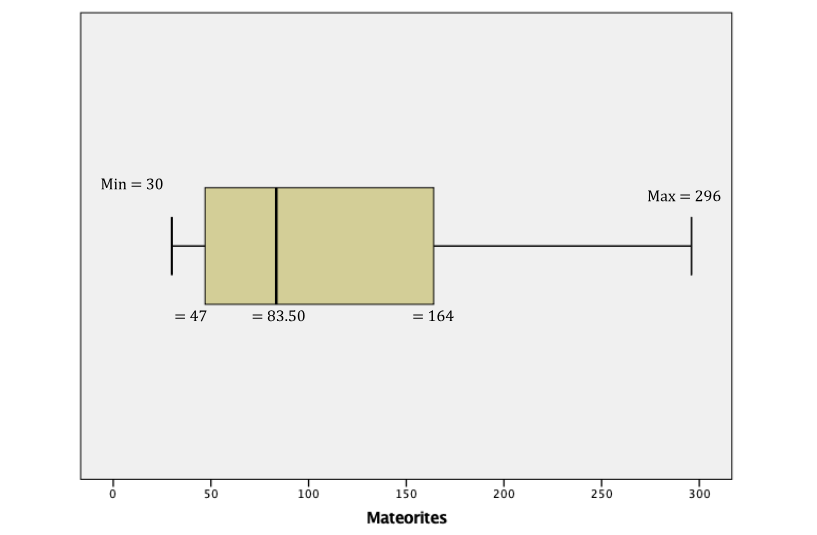
\includegraphics[width=4.16667in,height=\textheight]{images/ch2/picture17.png}

}

\caption{Figure 9: Skewed to the right / right skewness / positively
skewed}

\end{figure}

{\textbf{Example 2.15}}

A meteorologist is studying the monthly rainfall patterns in two
different regions, Region A and Region B, over the past year. They have
collected data for 11 months (in mm). They determine the skewness of the
two regions based on box and whiskers plot.

{\textbf{Answer :}}

\begin{figure}

{\centering 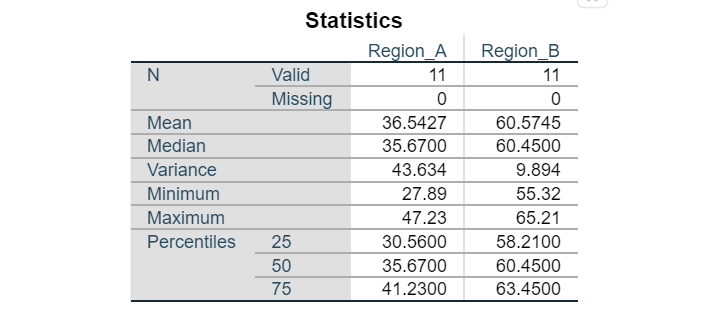
\includegraphics[width=4.16667in,height=\textheight]{images/ch2/picture18.png}

}

\caption{SPSS Output}

\end{figure}

\begin{figure}

{\centering 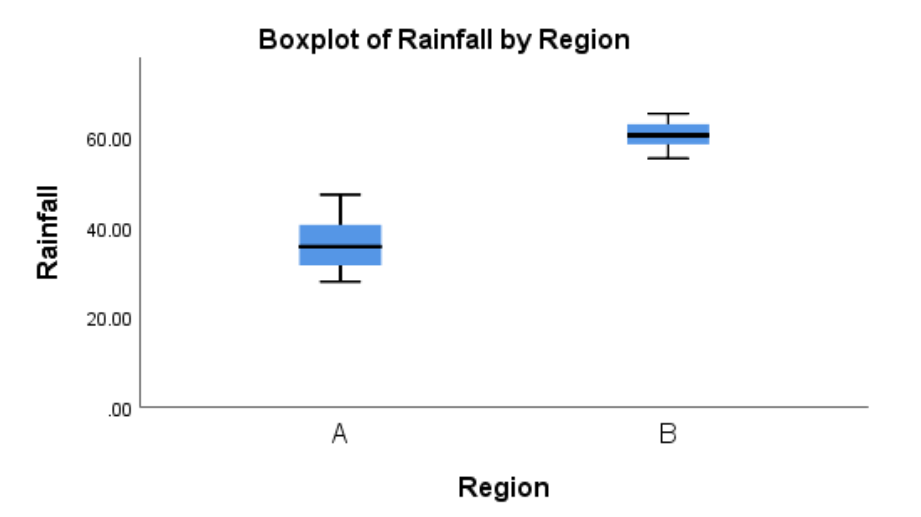
\includegraphics[width=5.20833in,height=\textheight]{images/ch2/picture19.png}

}

\caption{Figure 9: Region A -- positively skewed; Region B --
Approximately normal}

\end{figure}

\hypertarget{spss-output-on-numerical-descriptive-statistics}{%
\section{SPSS Output on Numerical Descriptive
Statistics}\label{spss-output-on-numerical-descriptive-statistics}}

IBM statistical software provides a wide range of statistical analysis
and graphing capabilities. We use dataset from SPSS's samples so that
students can have free access to it and be able to run it by themselves
to produce the SPSS output on descriptive statistics.

Data: \textbf{aflatoxin20.sav} Description: This data consists of 32
poison concentrations which are measured in parts per billion (PPB) on
corn crops. This poison is known as aflatoxin. The concentration varies
widely within crop yields.

To open a data file: From the menus choose: File \textgreater{} Open
\textgreater{} Data\ldots{} A dialog box for opening files is displayed
and choose \textbf{aflatoxin20.sav}

To obtain the descriptive analysis of the data:\\
1. From the menus choose:\\
Analyze \textgreater{} Descriptive Statistics \textgreater{}
Frequencies\ldots{}\\
The Frequencies dialog box is displayed.\\
2. Double click on \textbf{\emph{Aflatoxin PPB {[}toxin{]}}}\\
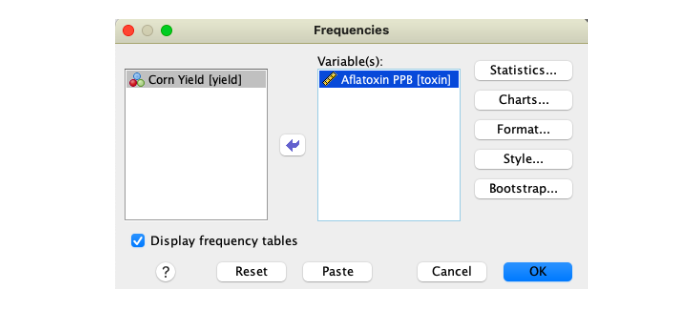
\includegraphics{images/ch2/picture20.png}\\
3. Click on \textbf{Statistics} and choose as per figure below:\\
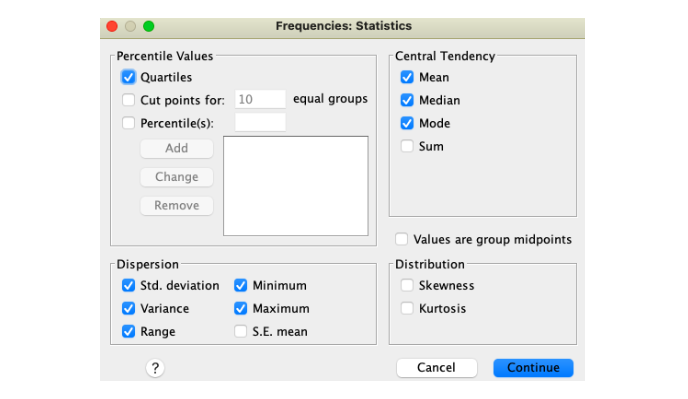
\includegraphics{images/ch2/picture21.png}\\
4. Click \textbf{Continue}\\
5. Click \textbf{OK} to run the procedure. Results are displayed in the
Viewer window.\\
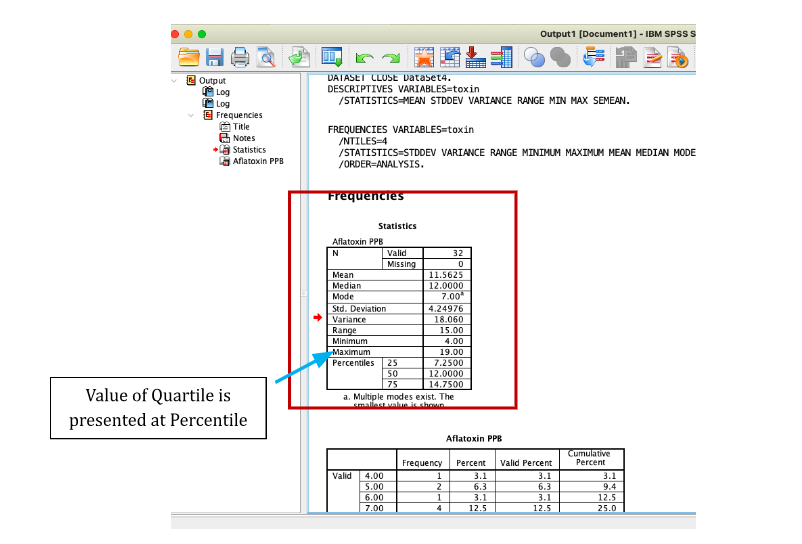
\includegraphics{images/ch2/picture22.png}\\

\hypertarget{exercise-2}{%
\section{Exercise 2}\label{exercise-2}}

\begin{enumerate}
\def\labelenumi{\arabic{enumi}.}
\tightlist
\item
  The weight (kg) of 12 customers registered for WX fitness studio are
  as follows.

  110, 90, 65, 100, 95, 75, 90, 85, 80, 70, 75, 90
\end{enumerate}

\begin{enumerate}
\def\labelenumi{\alph{enumi}.}
\tightlist
\item
  Find the mode and comment on the value obtained.
\item
  Calculate the mean and standard deviation.
\item
  Describe the shape of distribution by using an appropriate
  measurement.
\end{enumerate}

\begin{enumerate}
\def\labelenumi{\arabic{enumi}.}
\setcounter{enumi}{1}
\tightlist
\item
  A researcher studied petrol usage (in littles) for 14 cars travelling
  from town A to town B in a month. The data collected is shown below:

  81, 80, 65, 105, 144, 75, 150, 96, 91, 68, 135, 134, 95, 124
\end{enumerate}

\begin{enumerate}
\def\labelenumi{\alph{enumi}.}
\tightlist
\item
  Find the first quartile, median, and third quartile.
\item
  Construct a box-and-whiskers plot for the above data.
\item
  Determine the shape of the data distribution based on the
  box-and-whiskers plot.
\end{enumerate}

\begin{enumerate}
\def\labelenumi{\arabic{enumi}.}
\setcounter{enumi}{2}
\tightlist
\item
  The number of current issues books sold in a week by 12 bookstores at
  town A is as follows.

  11, 23, 12, 15, 22, 10, 16, 15, 7, 12, 26, 14
\end{enumerate}

\begin{enumerate}
\def\labelenumi{\alph{enumi}.}
\tightlist
\item
  Find the mean and the mode.
\item
  By comparing the mean and the mode in (a), determine the shape of the
  distribution for the above data.
\item
  Calculate the first quartile, median and third quartile of the above
  data.
\end{enumerate}

\begin{enumerate}
\def\labelenumi{\arabic{enumi}.}
\setcounter{enumi}{3}
\tightlist
\item
  The chemistry test marks of eight randomly selected students are given
  below:

  85, 65, 48, 70, 30, 80, 92, 70
\end{enumerate}

\begin{enumerate}
\def\labelenumi{\alph{enumi}.}
\tightlist
\item
  Calculate the mean, median and mode for the test score.
\item
  Find the variance of the test score for the selected students.
\item
  Determine the shape of the distribution of the test score using
  Pearson's coefficient of skewness.
\end{enumerate}

\begin{enumerate}
\def\labelenumi{\arabic{enumi}.}
\setcounter{enumi}{4}
\tightlist
\item
  The output below refers to National unemployment rate prior to the
  coronavirus outbreak (Covid-19).

  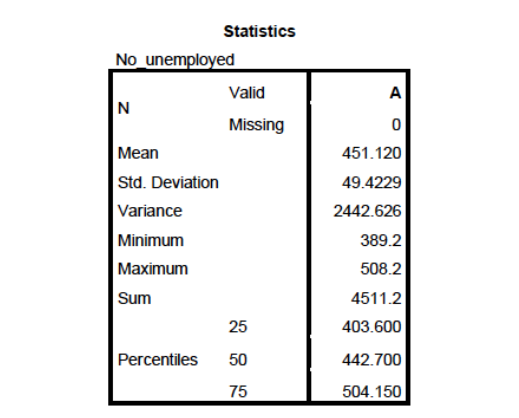
\includegraphics[width=4.16667in,height=\textheight]{images/ch2/picture23.png}
\end{enumerate}

\begin{enumerate}
\def\labelenumi{\alph{enumi}.}
\tightlist
\item
  Determine the value of \textbf{A}.
\item
  Find the value of Pearson Coefficient of Skewness. Then, identify the
  shape of distribution.
\item
  Based on information given in the output, sketch the appropriate
  diagram to represent the shape of distribution for unemployment rate.
\end{enumerate}

\begin{enumerate}
\def\labelenumi{\arabic{enumi}.}
\setcounter{enumi}{5}
\tightlist
\item
  A company is considering installing a new machine to assemble its
  product. The company is considering two types of machines, but it will
  buy only one type. The company selected eight assembly workers and
  asked them to use these two types of machines to assemble products.
  The data for two random samples is shown in Table 1. Table 2 shows the
  summary of the statistics for the time taken for the two types of
  machines based on data in Table 1.
\end{enumerate}

Table 1: Time taken (in minutes) to assemble one unit of product on each
machine

\begin{longtable}[]{@{}
  >{\raggedright\arraybackslash}p{(\columnwidth - 16\tabcolsep) * \real{0.2222}}
  >{\raggedright\arraybackslash}p{(\columnwidth - 16\tabcolsep) * \real{0.0694}}
  >{\raggedright\arraybackslash}p{(\columnwidth - 16\tabcolsep) * \real{0.0694}}
  >{\raggedright\arraybackslash}p{(\columnwidth - 16\tabcolsep) * \real{0.0694}}
  >{\raggedright\arraybackslash}p{(\columnwidth - 16\tabcolsep) * \real{0.0694}}
  >{\raggedright\arraybackslash}p{(\columnwidth - 16\tabcolsep) * \real{0.0694}}
  >{\raggedright\arraybackslash}p{(\columnwidth - 16\tabcolsep) * \real{0.0694}}
  >{\raggedright\arraybackslash}p{(\columnwidth - 16\tabcolsep) * \real{0.0694}}
  >{\raggedright\arraybackslash}p{(\columnwidth - 16\tabcolsep) * \real{0.0694}}@{}}
\toprule\noalign{}
\endhead
\bottomrule\noalign{}
\endlastfoot
\textbf{Machine 1} & 23 & 26 & 19 & 24 & 27 & 22 & 20 & 18 \\
\textbf{Machine 2} & 21 & 24 & 23 & 25 & 24 & 28 & 24 & 23 \\
\end{longtable}

Table 2: Summary Statistics
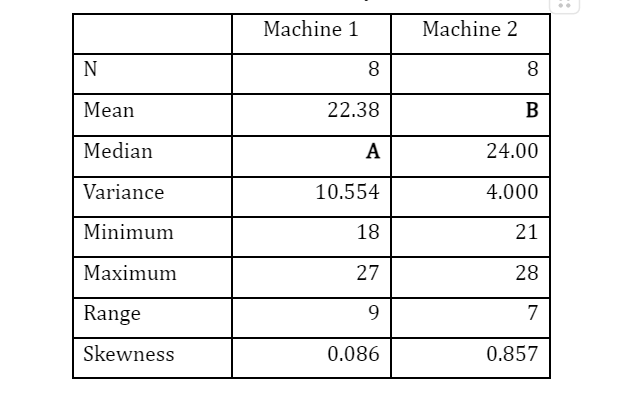
\includegraphics[width=4.16667in,height=\textheight]{images/ch2/picture24.png}

\begin{enumerate}
\def\labelenumi{\alph{enumi}.}
\tightlist
\item
  Compute the value of \textbf{A} and \textbf{B}.
\item
  Determine which machine is more consistent in their time taken to
  assemble one-unit product.
\end{enumerate}

\begin{enumerate}
\def\labelenumi{\arabic{enumi}.}
\setcounter{enumi}{6}
\tightlist
\item
  The weight of chickens (in kg) in small poultry in Klebang were
  summarize as follows:

  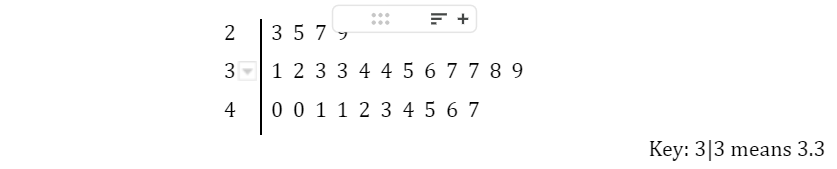
\includegraphics[width=7.29167in,height=\textheight]{images/ch2/picture25.png}
\end{enumerate}

\begin{enumerate}
\def\labelenumi{\alph{enumi}.}
\tightlist
\item
  Calculate the mean and standard deviation.
\item
  Determine the median value.
\item
  Interpret the value obtain in (b).
\item
  State the name of the plot.
\end{enumerate}

\hypertarget{answers-to-exercise-2}{%
\section{Answers to Exercise 2}\label{answers-to-exercise-2}}

\begin{enumerate}
\def\labelenumi{\arabic{enumi}.}
\item
  \begin{enumerate}
  \def\labelenumii{\alph{enumii})}
  \tightlist
  \item
    Mode = 90 kg. Most frequently weight of the customers for WX fitness
    studio is 90 kg.
  \item
    Mean = 85.42, s = 13.0486
  \item
    PMS = -0.3510. The distribution of data is skewed to the left.
  \end{enumerate}
\item
  \begin{enumerate}
  \def\labelenumii{\alph{enumii})}
  \tightlist
  \item
    Median (Q2) = 95.5, Q1 = 78.75, Q3 = 134.25
  \item
    The shape of the data distribution is skewed to the right.
  \end{enumerate}
\item
  \begin{enumerate}
  \def\labelenumii{\alph{enumii})}
  \tightlist
  \item
    Mean = 15.25, Mode = 12 and 15
  \item
    Since Mean \textgreater{} Mode, the shape of the distribution for
    the above data is skewed to the right.
  \item
    Q1 = 11.25, Q2 = 14.5, Q3 = 20.5
  \end{enumerate}
\item
  \begin{enumerate}
  \def\labelenumii{\alph{enumii})}
  \tightlist
  \item
    Mean = 67.5, median = 70, Mode = 70.
  \item
    Variance = 409.714
  \item
    PCS = -0.1235. The shape of the distribution of the test score is
    skewed to the left.
  \end{enumerate}
\item
  \begin{enumerate}
  \def\labelenumii{\alph{enumii})}
  \tightlist
  \item
    A = 10
  \item
    PCS = 0.5111 (positive skewness)
  \item
    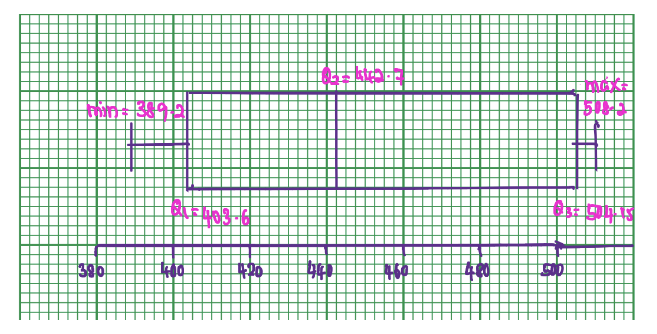
\includegraphics[width=4.16667in,height=\textheight]{images/ch2/picture26.png}
  \end{enumerate}
\end{enumerate}

6 a) A = 22.5; B = 24.0 b) CV1 = 14.52\%; CV2 = 8.33\% c) Machine 2 is
more consistent in time taken to assemble one unit of product compared
to Machine 1.

\begin{enumerate}
\def\labelenumi{\arabic{enumi}.}
\setcounter{enumi}{6}
\item
  \begin{enumerate}
  \def\labelenumii{\alph{enumii})}
  \tightlist
  \item
    Mean = 3.71 kg, s = 0.7022
  \item
    Median = 3.65 kg
  \item
    Half of the chicken's weights are less than 3.65kg and another half
    of the chickens weigh more than 3.65 kg.
  \item
    Stem and leaf plot.
  \end{enumerate}
\end{enumerate}

\hypertarget{tutorial-2}{%
\section{Tutorial 2}\label{tutorial-2}}

\begin{enumerate}
\def\labelenumi{\arabic{enumi}.}
\tightlist
\item
  The descriptive statistics for the life span (in years) of brand AA
  washing machine are summarized as below.
\end{enumerate}

Descriptive Statistics

\begin{longtable}[]{@{}
  >{\raggedright\arraybackslash}p{(\columnwidth - 12\tabcolsep) * \real{0.2500}}
  >{\raggedright\arraybackslash}p{(\columnwidth - 12\tabcolsep) * \real{0.0500}}
  >{\raggedright\arraybackslash}p{(\columnwidth - 12\tabcolsep) * \real{0.0875}}
  >{\raggedright\arraybackslash}p{(\columnwidth - 12\tabcolsep) * \real{0.0875}}
  >{\raggedright\arraybackslash}p{(\columnwidth - 12\tabcolsep) * \real{0.2125}}
  >{\raggedright\arraybackslash}p{(\columnwidth - 12\tabcolsep) * \real{0.1250}}
  >{\raggedright\arraybackslash}p{(\columnwidth - 12\tabcolsep) * \real{0.1250}}@{}}
\toprule\noalign{}
\endhead
\bottomrule\noalign{}
\endlastfoot
& N & Mean & Mode & Std. Deviation & Minimum & Maximum \\
Life span (years) & 89 & 6.59 & 7.04 & 0.74 & 5.2 & 8.1 \\
\end{longtable}

\begin{enumerate}
\def\labelenumi{\alph{enumi}.}
\tightlist
\item
  Calculate the coefficient of skewness. Hence, comment on the shape of
  the distribution.
\item
  Explain the meaning of the mode value.
\item
  Given the mean and variance for the life span (in years) of brand BB
  were 7.1 and 12.3 respectively. Using an appropriate measurement,
  determine which brand has a more consistent life span.
\end{enumerate}

\begin{enumerate}
\def\labelenumi{\arabic{enumi}.}
\setcounter{enumi}{2}
\tightlist
\item
  Waiting times (in minutes) of customers at the Providence Bank (PB)
  and the Valley Bank (VB) are given as follows.
\end{enumerate}

\begin{longtable}[]{@{}
  >{\raggedright\arraybackslash}p{(\columnwidth - 30\tabcolsep) * \real{0.0485}}
  >{\raggedright\arraybackslash}p{(\columnwidth - 30\tabcolsep) * \real{0.0583}}
  >{\raggedright\arraybackslash}p{(\columnwidth - 30\tabcolsep) * \real{0.0583}}
  >{\raggedright\arraybackslash}p{(\columnwidth - 30\tabcolsep) * \real{0.0583}}
  >{\raggedright\arraybackslash}p{(\columnwidth - 30\tabcolsep) * \real{0.0583}}
  >{\raggedright\arraybackslash}p{(\columnwidth - 30\tabcolsep) * \real{0.0583}}
  >{\raggedright\arraybackslash}p{(\columnwidth - 30\tabcolsep) * \real{0.0583}}
  >{\raggedright\arraybackslash}p{(\columnwidth - 30\tabcolsep) * \real{0.0583}}
  >{\raggedright\arraybackslash}p{(\columnwidth - 30\tabcolsep) * \real{0.0583}}
  >{\raggedright\arraybackslash}p{(\columnwidth - 30\tabcolsep) * \real{0.0583}}
  >{\raggedright\arraybackslash}p{(\columnwidth - 30\tabcolsep) * \real{0.0583}}
  >{\raggedright\arraybackslash}p{(\columnwidth - 30\tabcolsep) * \real{0.0485}}
  >{\raggedright\arraybackslash}p{(\columnwidth - 30\tabcolsep) * \real{0.0485}}
  >{\raggedright\arraybackslash}p{(\columnwidth - 30\tabcolsep) * \real{0.0485}}
  >{\raggedright\arraybackslash}p{(\columnwidth - 30\tabcolsep) * \real{0.0485}}
  >{\raggedright\arraybackslash}p{(\columnwidth - 30\tabcolsep) * \real{0.0388}}@{}}
\toprule\noalign{}
\endhead
\bottomrule\noalign{}
\endlastfoot
PB & 3.2 & 4.4 & 4.8 & 5.2 & 6.2 & 6.7 & 7.5 & 8.0 & 6.5 & 9.0 & 5.1 &
3.3 & 5.2 & 4.0 & 4.9 \\
VB & 5.8 & 5.6 & 5.7 & 5.8 & 6.1 & 6.4 & 6.7 & 6.7 & 6.7 & 6.8 & 6.5 &
7.0 & 6.9 & 6.5 & 6.4 \\
\end{longtable}

\begin{enumerate}
\def\labelenumi{\alph{enumi}.}
\tightlist
\item
  Calculate the mean and standard deviation for Valley Bank waiting
  times.
\item
  From the above box-and-whisker plots of waiting times for both
  Providence and Valley banks, comment on the shape of distribution for
  each plot.
\item
  The mean and standard deviation for Providence Bank are 5.6 and 1.692
  respectively. Determine which bank shows a more consistent wait time.
\end{enumerate}

\begin{enumerate}
\def\labelenumi{\arabic{enumi}.}
\setcounter{enumi}{2}
\tightlist
\item
  The stem and leaf plot below represents the History test scores (out
  of 100) of 15 randomly selected students in Class A.
\end{enumerate}

\begin{figure}

{\centering 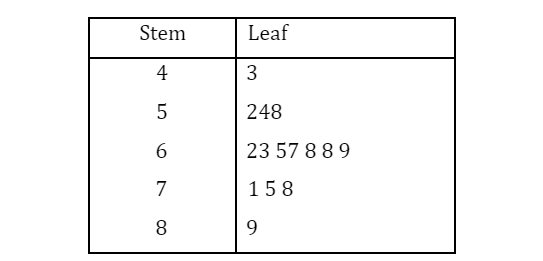
\includegraphics[width=5.20833in,height=\textheight]{images/ch2/picture27.png}

}

\caption{Key: 4\textbar3 means 43}

\end{figure}

\begin{enumerate}
\def\labelenumi{\alph{enumi}.}
\tightlist
\item
  Calculate the mean and standard deviation for the test score.
\item
  Interpret the mean obtained in a).
\item
  The summary statistics of the test score for History and Geography
  students in Class A are summarized in the following table. Using an
  appropriate measure, determine which distribution of the test score
  between the subjects is more dispersed.
\end{enumerate}

Descriptive statistics

\begin{longtable}[]{@{}
  >{\raggedright\arraybackslash}p{(\columnwidth - 6\tabcolsep) * \real{0.2222}}
  >{\raggedright\arraybackslash}p{(\columnwidth - 6\tabcolsep) * \real{0.1111}}
  >{\raggedright\arraybackslash}p{(\columnwidth - 6\tabcolsep) * \real{0.1528}}
  >{\raggedright\arraybackslash}p{(\columnwidth - 6\tabcolsep) * \real{0.2917}}@{}}
\toprule\noalign{}
\endhead
\bottomrule\noalign{}
\endlastfoot
& \textbf{N} & \textbf{Mean} & \textbf{Std. Deviation} \\
\textbf{History} & 15 & 65.4667 & 11.1859 \\
\textbf{Geography} & 17 & 66.9412 & 17.5623 \\
\end{longtable}

\begin{enumerate}
\def\labelenumi{\arabic{enumi}.}
\setcounter{enumi}{3}
\tightlist
\item
  The following chart shows the recorded weekly milk yield (in the
  nearest kg) for each cow selected at random from Farm A.
\end{enumerate}

\begin{figure}

{\centering 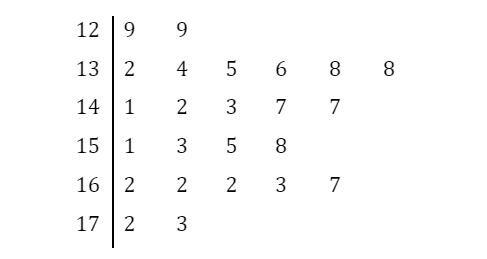
\includegraphics[width=5.20833in,height=\textheight]{images/ch2/picture28.png}

}

\caption{Key: 12\textbar9 means 129}

\end{figure}

\begin{enumerate}
\def\labelenumi{\alph{enumi}.}
\tightlist
\item
  State the name of the above chart.
\item
  Find the median weekly milk yield recorded at Farm A. Hence, interpret
  the result.
\item
  The statistics for the weekly milk yields for Farm A and Farm B are
  summarized in the following table. Using an appropriate measure,
  determine which farm has more consistent weekly milk yield.
\end{enumerate}

Descriptive statistics

\begin{longtable}[]{@{}
  >{\raggedright\arraybackslash}p{(\columnwidth - 6\tabcolsep) * \real{0.1806}}
  >{\raggedright\arraybackslash}p{(\columnwidth - 6\tabcolsep) * \real{0.1111}}
  >{\raggedright\arraybackslash}p{(\columnwidth - 6\tabcolsep) * \real{0.1528}}
  >{\raggedright\arraybackslash}p{(\columnwidth - 6\tabcolsep) * \real{0.2917}}@{}}
\toprule\noalign{}
\endhead
\bottomrule\noalign{}
\endlastfoot
& \textbf{N} & \textbf{Mean} & \textbf{Std. Deviation} \\
\textbf{Farm A} & 24 & 148.7 & 13.7 \\
\textbf{Farm B} & 28 & 158.5 & 8.33 \\
\end{longtable}

\begin{enumerate}
\def\labelenumi{\arabic{enumi}.}
\setcounter{enumi}{4}
\tightlist
\item
  The following chart summarizes the weight in kilograms of 17 male and
  female Orang Utans in the Reserves Centre.
\end{enumerate}

\begin{longtable}[]{@{}
  >{\raggedright\arraybackslash}p{(\columnwidth - 8\tabcolsep) * \real{0.1711}}
  >{\raggedright\arraybackslash}p{(\columnwidth - 8\tabcolsep) * \real{0.1447}}
  >{\raggedright\arraybackslash}p{(\columnwidth - 8\tabcolsep) * \real{0.2763}}
  >{\raggedright\arraybackslash}p{(\columnwidth - 8\tabcolsep) * \real{0.1842}}
  >{\raggedright\arraybackslash}p{(\columnwidth - 8\tabcolsep) * \real{0.1842}}@{}}
\toprule\noalign{}
\endhead
\bottomrule\noalign{}
\endlastfoot
\textbf{Gender} & \textbf{Mean} & \textbf{Std. Deviation} &
\textbf{Minimum} & \textbf{Maximum} \\
Male & 117.94 & 13.32 & 100 & 150 \\
Female & 97.65 & 17.79 & 65 & 120 \\
\end{longtable}

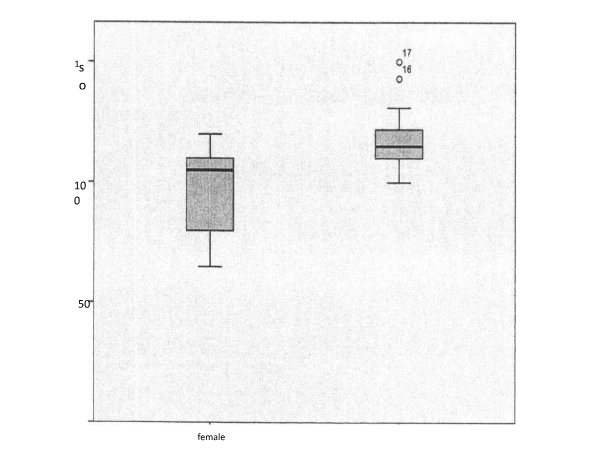
\includegraphics[width=5.20833in,height=\textheight]{images/ch2/picture29.png}

\begin{enumerate}
\def\labelenumi{\alph{enumi}.}
\tightlist
\item
  Name the diagram given.
\item
  Identify the outlier(s), if any.
\item
  Using an appropriate measure, determine which gender is more
  consistent in distribution of weight.
\end{enumerate}

\begin{enumerate}
\def\labelenumi{\arabic{enumi}.}
\setcounter{enumi}{5}
\tightlist
\item
  The weekly consumption of cheese (in ounces) for 35 participants in a
  nutrition study is summarize as follows:
\end{enumerate}

\begin{longtable}[]{@{}
  >{\raggedright\arraybackslash}p{(\columnwidth - 8\tabcolsep) * \real{0.2917}}
  >{\raggedright\arraybackslash}p{(\columnwidth - 8\tabcolsep) * \real{0.0556}}
  >{\raggedright\arraybackslash}p{(\columnwidth - 8\tabcolsep) * \real{0.1667}}
  >{\raggedright\arraybackslash}p{(\columnwidth - 8\tabcolsep) * \real{0.1944}}
  >{\raggedright\arraybackslash}p{(\columnwidth - 8\tabcolsep) * \real{0.0556}}@{}}
\toprule\noalign{}
\endhead
\bottomrule\noalign{}
\endlastfoot
& N & \(\sum{x}\) & \(\sum{x^2}\) & W \\
Cheese (in ounces) & 25 & 265 & 4579 & 10 \\
\end{longtable}

\begin{enumerate}
\def\labelenumi{\alph{enumi}.}
\tightlist
\item
  Calculate the mean and standard deviation
\item
  Most participants spent 10 ounces of cheese weekly. Based on the given
  interpretation, name the statistical measure of W.
\item
  Identify the skewness of the weekly consumption of cheese using
  appropriate measurement.
\end{enumerate}

\hypertarget{answers-to-tutorial-2}{%
\section{Answers to Tutorial 2}\label{answers-to-tutorial-2}}

1 a) Coefficient of skewness = -0.6081 The shape of the distribution is
skewed to the left. b) Mode =7.04 Most of the life span of Brand AA
washing machine is 7.04 years. c) CV for Brand AA = 11.23\%, CV for
Brand BB = 49.40\% Therefore, Brand AA has a more consistent of life
span.

\begin{enumerate}
\def\labelenumi{\arabic{enumi}.}
\setcounter{enumi}{1}
\item
  \begin{enumerate}
  \def\labelenumii{\alph{enumii})}
  \tightlist
  \item
    Mean = 6.373, s = 0.462
  \item
    The shape of the distribution of PB is skewed to the right. The
    shape of the distribution of VB is skewed to the left.
  \end{enumerate}
\item
  \begin{enumerate}
  \def\labelenumii{\alph{enumii})}
  \tightlist
  \item
    Mean = 65.467, n = 15, s = 11.186
  \item
    The average test score of History is 65.467.
  \item
    History test scores is more consistent the Geography test scores.
  \end{enumerate}
\item
  \begin{enumerate}
  \def\labelenumii{\alph{enumii})}
  \tightlist
  \item
    Stem-and-Leaf Plot
  \item
    Median = 147 kg 50\% of the weekly milk yield is less than 147 kg.
  \item
    Farm B has more consistent weekly milk yield.
  \end{enumerate}
\item
  \begin{enumerate}
  \def\labelenumii{\alph{enumii})}
  \tightlist
  \item
    Box and Whisker Plot
  \item
    Outliers : 16, 17
  \item
    Male is more consistent in distribution of weight.
  \end{enumerate}
\item
  \begin{enumerate}
  \def\labelenumii{\alph{enumii})}
  \tightlist
  \item
    Mean = 10.6 ounces, s = 8.588
  \item
    Mode
  \item
    PCS = 0.07 (approximately normal)
  \end{enumerate}
\end{enumerate}

\bookmarksetup{startatroot}

\hypertarget{estimation}{%
\chapter{Estimation}\label{estimation}}

\hypertarget{learning-objectives-2}{%
\section*{Learning Objectives:}\label{learning-objectives-2}}
\addcontentsline{toc}{section}{Learning Objectives:}

\markright{Learning Objectives:}

\begin{enumerate}
\def\labelenumi{\arabic{enumi}.}
\tightlist
\item
  Describe and construct the interval estimation for the mean of the
  population parameter (both σ known and σ unknown) for \textbf{large
  and small sample size}.
\item
  Describe and construct the interval estimation for the difference
  between two means (both σ known and σ unknown) for
  \textbf{independent} sample.
\item
  Describe and construct the interval estimation for the difference
  between two means (both σ known and σ unknown) for \textbf{dependent}
  sample.
\end{enumerate}

\hypertarget{introduction-2}{%
\section{Introduction}\label{introduction-2}}

Estimation is the process in which a numerical value collected from a
sample is assigned to a population parameter. The value(s) that is
assigned to a population parameter based on the sample statistic is
called an estimation while the sample statistic used to estimate
population parameter is called an estimator. There are two (2) types of
estimates that will be discussed in this chapter name as point estimate
and interval estimate.

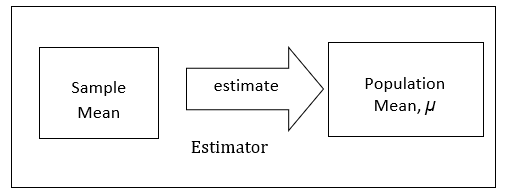
\includegraphics[width=5.20833in,height=\textheight]{images/ch3/picture1.png}

\hypertarget{point-estimation}{%
\section{Point Estimation}\label{point-estimation}}

A point estimate is a specific numerical value estimate of a parameter.

The value calculated from a sample mean, \(\bar{x}\) is the best point
estimate of the population mean, \(\mu\). In estimation, the calculation
margin of error is calculated based on point estimation.

\hypertarget{interval-estimation}{%
\section{\texorpdfstring{Interval Estimation\\
}{Interval Estimation }}\label{interval-estimation}}

\begin{itemize}
\tightlist
\item
  An \textbf{interval estimate} of a parameter is an \textbf{interval}
  or a \textbf{range} of values used to estimate the parameter based on
  observations from one sample. There are two (2) values in the interval
  estimate: \textbf{lower limit} and \textbf{upper limit}.\\
\item
  The interval constructed around the point estimate, but the estimate
  may or may not contain the value of the parameter being estimated.\\
\item
  Each interval constructed also regards a given confidence level and it
  is called a confidence interval.\\
\item
  A \textbf{confidence interval} is a specific interval estimate of a
  parameter determined by using data obtained from a sample and by using
  the specific confidence level of the estimate.\\
\item
  The \textbf{confidence level} of an interval estimate of a parameter
  is the probability that the interval estimate will contain the
  parameter. It is denoted by (1-)100\%. The is called a
  \textbf{significance level} (probability that the parameter is not
  within the interval).\\
\item
  In constructing a confidence interval, researchers can choose any
  value for confidence level for example 90\%, 95\% and 99\%.\\
\end{itemize}

\hypertarget{interval-estimate-for-a-mean-when-ux3c3-is-knownunknown}{%
\subsection{Interval Estimate for a Mean (when σ is
Known/Unknown)}\label{interval-estimate-for-a-mean-when-ux3c3-is-knownunknown}}

\hypertarget{case-1-confidence-interval-of-the-mean-for-ux3c3-is-known-and-large-sample-size-n-30}{%
\subsubsection{\texorpdfstring{\textbf{CASE 1: Confidence Interval of
the Mean for σ is Known and Large Sample Size (n ≥
30)}}{CASE 1: Confidence Interval of the Mean for σ is Known and Large Sample Size (n ≥ 30)}}\label{case-1-confidence-interval-of-the-mean-for-ux3c3-is-known-and-large-sample-size-n-30}}

\(\bar{X} – Z_{\frac{\alpha}{2}}\left(\frac{\sigma}{\sqrt{n}}\right) \lt \mu \lt \bar{X} + Z_{\frac{\alpha}{2}}\left(\frac{\sigma}{\sqrt{n}}\right)\ \ \ \ \ or\ \ \ \ \ \ \bar{X} \pm Z_{\frac{\alpha}{2}}\left(\frac{\sigma}{\sqrt{n}}\right)\)

\begin{tcolorbox}[enhanced jigsaw, arc=.35mm, bottomtitle=1mm, coltitle=black, colbacktitle=quarto-callout-tip-color!10!white, rightrule=.15mm, colframe=quarto-callout-tip-color-frame, toptitle=1mm, opacityback=0, colback=white, breakable, titlerule=0mm, title=\textcolor{quarto-callout-tip-color}{\faLightbulb}\hspace{0.5em}{Tip}, opacitybacktitle=0.6, leftrule=.75mm, bottomrule=.15mm, toprule=.15mm, left=2mm]

For a 90\% confidence interval: \(z_{α/2}=1.65\)~\\
For a 95\% confidence interval: \(z_{α/2}=1.96\)\\
For a 99\% confidence interval: \(z_{α/2}=2.58\)\\

\marginnote{\begin{footnotesize}

{Note:} To determine the value of z, please refer to \textbf{Table 3} or
\textbf{Table 4} from Statistical Tables.

\end{footnotesize}}

\end{tcolorbox}

{\textbf{Example 3.1}}

95\% Confidence Interval of the Mean

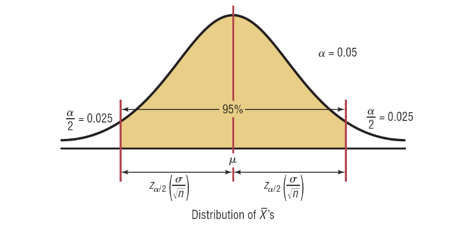
\includegraphics[width=5.20833in,height=\textheight]{images/ch3/picture2.png}

Refer Table 3 or Table 4 to determine the value of z.

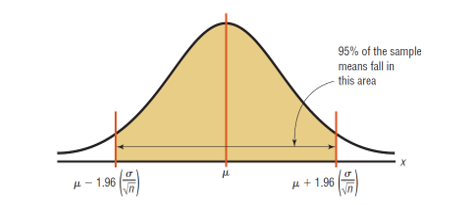
\includegraphics[width=5.20833in,height=\textheight]{images/ch3/picture3.png}

{\textbf{Example 3.2}}

A researcher wishes to estimate the number of days it takes an
automobile dealer to sell Aza Aveo. A sample of 50 cars had a mean time
on the dealer's lot of 54 days. Assume the population standard deviation
to be 6.0 days. Find the best point estimate of the population mean and
the 95\% confidence interval of the population mean.

{\textbf{Answer:}}

The best point estimate of the mean (\(\mu\)) is 54 days.

Given:

\(\bar{X} = 54,\ \sigma = 6.0,\ n = 50, 95\%\ confident\ level\ \rightarrow z = 1.96\)

95\% confidence interval of the population mean:\\

\[
\begin{aligned}
\bar{X} – Z_{\frac{\alpha}{2}}\left(\frac{\sigma}{\sqrt{n}}\right) &\lt \mu \lt \bar{X} + Z_{\frac{\alpha}{2}}\left(\frac{\sigma}{\sqrt{n}}\right) \\
54 – 1.96\Bigg(\frac{60}{\sqrt{50}}\right) &\lt \mu \lt 54 + 1.96\left(\frac{60}{\sqrt{50}}\right) \\
54 - 1.663 &\lt \mu \lt 54 + 1.663 \\
52.337 &\lt \mu \lt 55.663
\end{aligned}
\]

\hfill\break
\hfill\break
\hfill\break
or

\[
\begin{aligned}
\bar{X} &\pm Z_{\frac{\alpha}{2}}\left(\frac{\sigma}{\sqrt{n}}\right) \\
54 &\pm 1.96\left(\frac{60}{\sqrt{50}}\right)\\
54 &\pm 1.663 \\
(52.337&,\ 55.663)
\end{aligned}
\]

One can say with 95\% confidence that the interval between 52 and 56
days contains the population mean, based on a sample of 50 automobiles.

{\textbf{Example 3.3}}

A large department store found that it averages 362 customers per hour.
Assume that the standard deviation is 29.6 and a random sample of 40
hours was used to determine the average. Find the 99\% confidence
interval of the population mean.

{\textbf{Answer:}}

\[
\begin{aligned}
\bar{X} – Z_{\frac{\alpha}{2}}\left(\frac{\sigma}{\sqrt{n}}\right) &\lt \mu \lt \bar{X} + Z_{\frac{\alpha}{2}}\left(\frac{\sigma}{\sqrt{n}}\right) \\
362 – 2.58\left(\frac{29.6}{\sqrt{40}}\right) &\lt \mu \lt 362 + 2.58\left(\frac{29.6}{\sqrt{40}}\right) \\
362 - 12.1 &\lt \mu \lt 362 + 12.1 \\
349.9 &\lt \mu \lt 374.1
\end{aligned}
\]

\hfill\break
\hfill\break
\hfill\break
or

\[
\begin{aligned}
\bar{X} &\pm Z_{\frac{\alpha}{2}}\left(\frac{\sigma}{\sqrt{n}}\right) \\
362 &\pm 2.58\left(\frac{29.6}{\sqrt{40}}\right)\\
362 &\pm 12.1 \\
(349.9&,\ 374.1)
\end{aligned}
\]

Hence, one can be 99\% confident that the mean number of customers that
the store averages is between 350 and 374 customers per hour (rounding
values).

\hypertarget{case-2-confidence-interval-of-the-mean-for-sigma-is-unknown-and-large-sample-size-n-ge-30}{%
\subsubsection{\texorpdfstring{\textbf{CASE 2: Confidence Interval of
the Mean for \(\sigma\) is Unknown and Large Sample Size
(\(n \ge 30\))}}{CASE 2: Confidence Interval of the Mean for \textbackslash sigma is Unknown and Large Sample Size (n \textbackslash ge 30)}}\label{case-2-confidence-interval-of-the-mean-for-sigma-is-unknown-and-large-sample-size-n-ge-30}}

\[
\bar{X} – Z_{\frac{\alpha}{2}}\left(\frac{s}{\sqrt{n}}\right) \lt \mu \lt \bar{X} + Z_{\frac{\alpha}{2}}\left(\frac{s}{\sqrt{n}}\right)\ \ \ \ \ or\ \ \ \ \ \ \bar{X} \pm Z_{\frac{\alpha}{2}}\left(\frac{s}{\sqrt{n}}\right)
\]

{\textbf{Example 3.4}}

The following data represent a sample of the assets (in millions of
ringgit Malaysia) of 30 credit banks in Malaysia. Find the 90\%
confidence interval of the mean. Given standard deviation for the
following data is 14.405.\\

\begin{longtable}[]{@{}
  >{\raggedright\arraybackslash}p{(\columnwidth - 18\tabcolsep) * \real{0.0833}}
  >{\raggedright\arraybackslash}p{(\columnwidth - 18\tabcolsep) * \real{0.0833}}
  >{\raggedright\arraybackslash}p{(\columnwidth - 18\tabcolsep) * \real{0.0833}}
  >{\raggedright\arraybackslash}p{(\columnwidth - 18\tabcolsep) * \real{0.0833}}
  >{\raggedright\arraybackslash}p{(\columnwidth - 18\tabcolsep) * \real{0.0694}}
  >{\raggedright\arraybackslash}p{(\columnwidth - 18\tabcolsep) * \real{0.0694}}
  >{\raggedright\arraybackslash}p{(\columnwidth - 18\tabcolsep) * \real{0.0833}}
  >{\raggedright\arraybackslash}p{(\columnwidth - 18\tabcolsep) * \real{0.0833}}
  >{\raggedright\arraybackslash}p{(\columnwidth - 18\tabcolsep) * \real{0.0833}}
  >{\raggedright\arraybackslash}p{(\columnwidth - 18\tabcolsep) * \real{0.0833}}@{}}
\toprule\noalign{}
\endhead
\bottomrule\noalign{}
\endlastfoot
12.23 & 16.56 & 4.39 & 2.89 & 1.24 & 2.17 & 13.19 & 9.16 & 1.42 &
73.25 \\
1.91 & 14.64 & 11.59 & 6.69 & 1.06 & 8.74 & 3.17 & 18.13 & 7.92 &
4.78 \\
16.85 & 40.22 & 2.42 & 21.58 & 5.01 & 1.47 & 12.24 & 2.27 & 12.77 &
2.76 \\
\end{longtable}

\[
\begin{aligned}
\bar{X} – Z_{\frac{\alpha}{2}}\left(\frac{s}{\sqrt{n}}\right) &\lt \mu \lt \bar{X} + Z_{\frac{\alpha}{2}}\left(\frac{s}{\sqrt{n}}\right) \\
11.091 – 1.645\left(\frac{14.405}{\sqrt{30}}\right) &\lt \mu \lt 11.091 + 1.645\left(\frac{14.405}{\sqrt{30}}\right) \\
11.091 - 4.326 &\lt \mu \lt 11.091 + 4.326 \\
6.765 &\lt \mu \lt 15.417
\end{aligned}
\]

One can be 90\% confident that the population mean of the assets of all
credit unions is between RM6.765 million and RM15.417 million, based on
a sample of 30 credit unions.

\textbf{Output from SPSS}

Calculation based on the above output:

\[
\begin{aligned}
\bar{X} &\pm Z_{\frac{\alpha}{2}}\left(\frac{s}{\sqrt{n}}\right) \\
11.0907 &\pm 1.645\left(\frac{14.40545}{\sqrt{30}}\right)\\
11.0907 &\pm 1.645(2.63006) \\
11.0907 &\pm 4.3264 \\
(6.7643&,\ 15.4171)
\end{aligned}
\]

\hypertarget{case-3-confidence-interval-of-the-mean-for-sigma-is-unknown-and-small-sample-size-n-lt-30}{%
\subsubsection{\texorpdfstring{\textbf{CASE 3: Confidence Interval of
the Mean for \(\sigma\) is Unknown and Small Sample Size
(\(n \lt 30\))}}{CASE 3: Confidence Interval of the Mean for \textbackslash sigma is Unknown and Small Sample Size (n \textbackslash lt 30)}}\label{case-3-confidence-interval-of-the-mean-for-sigma-is-unknown-and-small-sample-size-n-lt-30}}

\[
\bar{X} – t_{\frac{\alpha}{2},df}\Bleft(\frac{s}{\sqrt{n}}\right) \lt \mu \lt \bar{X} + t_{\frac{\alpha}{2},df}\left(\frac{s}{\sqrt{n}}\right)\ \ \ \ \ or\ \ \ \ \ \ \bar{X} \pm t_{\frac{\alpha}{2},df}\left(\frac{s}{\sqrt{n}}\right)
\]

\marginnote{\begin{footnotesize}

The degrees of freedom (df) are \textbf{\(n-1\)}.\\
{Note:} Refer to \textbf{Table 7} from Statistical Table

\end{footnotesize}}

\begin{itemize}
\tightlist
\item
  The value of σ, when it is not known, must be estimated using the
  standard deviation (s) of the sample.
\item
  When standard deviation (s) is used, especially when the sample size
  is small (less than 30), critical values greater than the values for
  are used in confidence intervals to keep the interval at a given
  level, such as the 95\%.
\item
  These values are taken from the \textbf{Student
  \emph{t}-distribution,} most often called the
  \textbf{\emph{t}-distribution}.
\end{itemize}

\textbf{Characteristics of the t -distribution}

The t -distribution is like the standard normal distribution in these
ways:

\begin{itemize}
\tightlist
\item
  It is bell-shaped.
\item
  It is symmetric about the mean.
\item
  The mean, median, and mode are equal to 0 and are located at the
  center of the distribution.
\item
  The curve never touches the x-axis.
\end{itemize}

The t-distribution differs from the standard normal distribution in the
following ways:

\begin{itemize}
\tightlist
\item
  The variance is greater than 1.
\item
  The t-distribution is a family of curves based on the concept of
  \textbf{degrees of freedom} which is related to sample size.
\item
  As the sample size increases, the t-distribution approaches the
  standard normal distribution.
\end{itemize}

{\textbf{Example 3.5}}

A random sample of 10 children found that their average growth for the
first year was 9.8 inches. Assume the variable is normally distributed
and the sample standard deviation is 0.96 inch. Find the 95\% confidence
interval of the population mean for growth during the first year.

Given that \(\bar{X}=9.8, s=0.96, n=10, df=10-1=9\)

\[
\bar{X} – t_{\frac{\alpha}{2},df}\left(\frac{s}{\sqrt{n}}\right) \lt \mu \lt \bar{X} + t_{\frac{\alpha}{2},df}\left(\frac{s}{\sqrt{n}}\right) \\
9.8 – t_{\frac{0.05}{2},9}\left(\frac{0.96}{\sqrt{10}}\right) \lt \mu \lt 9.8 + t_{\frac{0.05}{2},9}\left(\frac{0.96}{\sqrt{10}}\right) \\
9.8 – 2.262\left(\frac{0.96}{\sqrt{10}}\right) \lt \mu \lt 9.8 + 2.262\left(\frac{0.96}{\sqrt{10}}\right) \\
9.11 \lt \mu \lt 10.49
\]

Therefore, one can be 95\% confident that the population mean of the
first-year growth is between 9.11 and 10.49 inches.

{\textbf{Example 3.6}}

The data represent a sample of the number of home fires started by
candles for the past seven (7) years. Find the 99\% confidence interval
for the mean number of home fires started by candles each year.

5460, 5900, 6090, 6310, 7160, 8440, 9930

\hfill\break

\textbf{Step 1}

Find the mean and standard deviation. The mean is \(\bar{x}\) = 7041.4
and standard deviation \(s\) = 1610.3.

\textbf{Step 2}

Find \(t_{\frac{\alpha}{2}}\) in Table 7. The confidence level is 99\%,
and the degrees of freedom \(df = 6\). \(t_{\frac{0.99}{2},6} = 3.707\).

\[
\bar{X} – t_{\frac{\alpha}{2},df}\ \left(\frac{s}{\sqrt{n}}\right) \lt \mu \lt \bar{X} + t_{\frac{\alpha}{2},df}\ \left(\frac{s}{\sqrt{n}}\right)\\
7041.4 – 3.707\ \left(\frac{1610.3}{\sqrt{7}}\right) \lt \mu \lt 7041.4 + 3.707\ \left(\frac{1610.3}{\sqrt{7}}\right)\\
7041.4 - 2256.21 \lt \mu \lt 7041.4 + 2256.21 \\
4785.19 \lt \mu \lt 9297.61
\]

One can be 99\% confident that the population mean number of home fires
started by candles each year is between 4785 and 9298, based on a sample
of home fires occurring over a period of 7 years.\\

\textbf{Output from SPSS for the above data}\\

\begin{figure}

{\centering 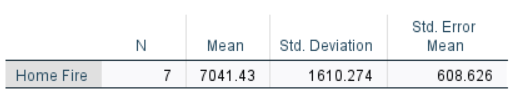
\includegraphics[width=4.16667in,height=\textheight]{images/ch3/table3_3.png}

}

\caption{Table 3.3: One Sample Statistics}

\end{figure}

\begin{figure}

{\centering \includegraphics[width=5.20833in,height=\textheight]{images/ch3/table3_4.png}

}

\caption{Table 3.4: One-Sample Test}

\end{figure}

\[
\bar{X} \pm t_{\frac{\alpha}{2},df}\left(\frac{s}{\sqrt{n}}\right),\ df=6\\
7041.43 \pm 3.707\left(\frac{1610.274}{\sqrt{7}}\right)\\
7041.43 \pm 2256.18 \\
(4785.25,\ 9297.61) \\
or
\]

From the SPSS output, 99\% confidence interval is (4784.99,9297.87).\\

\hypertarget{estimation-the-difference-between-two-means}{%
\subsection{\texorpdfstring{Estimation the Difference Between Two
Means\\
}{Estimation the Difference Between Two Means }}\label{estimation-the-difference-between-two-means}}

\textbf{CASE 1: Testing the Difference Between Two Means of Independent
Samples: Using the z Test}\\

Assumptions:\\

\begin{enumerate}
\def\labelenumi{\arabic{enumi}.}
\tightlist
\item
  Both samples are random samples.
\item
  The samples must be independent of each other. That is, there can be
  no relationship between the subjects in each sample.
\item
  The standard deviations of both populations must be known; and if the
  sample sizes are greater than 30, the populations must be normally or
  approximately normally distributed.
\end{enumerate}

\textbf{Confidence Intervals for the Difference Between Two Means of
Independent Samples: Large Samples}\\

Formula for the \(z\) confidence interval for the difference between two
means from independent populations\\

\begin{enumerate}
\def\labelenumi{\roman{enumi})}
\tightlist
\item
\end{enumerate}

\((\bar{X_1}-\bar{X_2})-Z_{\frac{\alpha}{2}}{\sqrt{\frac{\sigma_1^2}{n_1}+\frac{\sigma_2^2}{n_2}}}\lt(\mu_1-\mu_2)\lt(\bar{X_1}-\bar{X_2})+Z_{\frac{\alpha}{2}}{\sqrt{\frac{\sigma_1^2}{n_1}+\frac{\sigma_2^2}{n_2}}}\)\\
or,\\
\((\bar{X_1}-\bar{X_2})\pm Z_{\frac{\alpha}{2}}{\sqrt{\frac{\sigma_1^2}{n_1}+\frac{\sigma_2^2}{n_2}}}\)
\textbf{(when \(\sigma\) is known)}

\begin{enumerate}
\def\labelenumi{\roman{enumi})}
\setcounter{enumi}{1}
\tightlist
\item
\end{enumerate}

\((\bar{X_1}-\bar{X_2})-Z_{\frac{\alpha}{2}}{\sqrt{\frac{s_1^2}{n_1}+\frac{s_2^2}{n_2}}}\lt(\mu_1-\mu_2)\lt(\bar{X_1}-\bar{X_2})+Z_{\frac{\alpha}{2}}{\sqrt{\frac{s_1^2}{n_1}+\frac{s_2^2}{n_2}}}\)\\
or,\\
\((\bar{X_1}-\bar{X_2})\pm Z_{\frac{\alpha}{2}}{\sqrt{\frac{s_1^2}{n_1}+\frac{s_2^2}{n_2}}}\)
\textbf{(when \(\sigma\) is unknown)}

{\textbf{Example 3.7}}\\

A study using two random samples of 35 people each found that the
average amount of time those in the age group of 26--35 years spent per
week on leisure activities was 39.6 hours, and those in the age group of
46--55 years spent 35.4 hours. Assume that the population standard
deviation for those in the first and second age group found by previous
studies are 6.3 and 5.8 hours respectively. At \(\alpha\) = 0.05, find
the 95\% confidence interval for the difference between the means for
the data.\\

{\textbf{Answer}}\\

Given that
\(\bar{X-1}=39.6,\ \bar{X_2}=35.4,\ \sigma_1=6.3,\ \sigma_2=5.8,\ n_1=35,\ n_2=35\)\\

\[
\begin{aligned}
(\bar{X_1}-\bar{X_2})\ &\pm\ Z_{\frac{\alpha}{2}}{\sqrt{\frac{\sigma_1^2}{n_1}+\frac{\sigma_2^2}{n_2}}} \\
(39.6\ -\ 35.4)\ &\pm\ Z_{\frac{0.05}{2}}{\sqrt{\frac{6.3^2}{35}+\frac{5.8^2}{35}}} \\
4.2\ &\pm\ 1.96{\sqrt{\frac{6.3^2}{35}+\frac{5.8^2}{35}}} \\
&(1.363,\ 7.037)
\end{aligned}
\]

\begin{quote}
Interpretation:\\
With 95\% confident, there is significant different on the average
amount of time spent per week on leisure activities between the two-age
group since 0 value is not included in the interval.
\end{quote}

\textbf{CASE 2: Difference Between Two Means of Independent Samples:
\emph{Using the t-test} }\\

Assumptions:\\

\begin{enumerate}
\def\labelenumi{\arabic{enumi}.}
\tightlist
\item
  The samples are random samples.
\item
  The sample data are independent of one another.
\item
  When the sample sizes are less than 30, the populations must be
  normally or approximately normally distributed.\\
\end{enumerate}

The Independent t-test was used to compare the average values and
determine the significant difference in the means of the two groups. The
Independent t-test \textbf{assumes the variance of the two sample groups
are approximately equal or the samples have homogeneity of variance}.
The variance does not have too precisely equal but just close enough.
The homogeneity of variance means the two groups are of the same nature
or have the same kind of variability. To know if the variance is close
enough to be called homogeneous or not, the \textbf{Levene Test for
Equality of Variances} will be used.\\

The steps for conducting Levene Test using output from SPSS are as
follow:\\

Step 1:

Hypothesis\\
\(H_0:\ \sigma_1^2=\ \sigma_2^2\) (Equal variances)\\
\(H_1:\ \sigma_1^2\ne\ \sigma_2^2\) (Not equal variances)

Step 2:

\(\alpha\) value

Step 3:

\emph{p}-value

Step 4 \& 5:

Decision and conclusion.\\
If \emph{p}-value is greater than \(\alpha\) value, therefore the
variances are assumed to be equal. Otherwise, variances are assumed not
equal when \emph{p}-value is less than \(\alpha\) value.

\begin{tcolorbox}[enhanced jigsaw, arc=.35mm, bottomtitle=1mm, coltitle=black, colbacktitle=quarto-callout-note-color!10!white, rightrule=.15mm, colframe=quarto-callout-note-color-frame, toptitle=1mm, opacityback=0, colback=white, breakable, titlerule=0mm, title=\textcolor{quarto-callout-note-color}{\faInfo}\hspace{0.5em}{Note}, opacitybacktitle=0.6, leftrule=.75mm, bottomrule=.15mm, toprule=.15mm, left=2mm]

\begin{enumerate}
\def\labelenumi{(\alph{enumi})}
\tightlist
\item
  Confidence Intervals for the Difference Between Two Means (Difference
  in means of two normal distributions (independent populations), µ1 -
  µ2, variances equal and unknown)\\
\end{enumerate}

Small sample case with unknown but \textbf{equal standard deviation}\\

\begin{quote}
\(df=n_1 + n_2 -2\)\\
\((\bar{x_1}\ -\ \bar{x_2})\ \pm\ t_{\frac{\alpha}{2},\ df}\ s_p\sqrt{\frac{1}{n_1}\ +\ \frac{1}{n_2}}\)\\
where,
\(s_p\ =\ \sqrt{\frac{(n_1-1)s_1^2\ +\ (n_2-1)s_2^2}{n_1+n_2-2}}\)\\
\end{quote}

{\textbf{Example 3.8}}\\

Nowadays the nursing profession is very marketable profession in
Malaysia. A government hospital normally employs nurse who have been
trained from both the government and private training centers. The
hospital administrator is interested to determine which training centers
seem to educate its nurses better. The hospital devised a test to be
given to the newly graduated nurses entering the hospital. The scores
are as follows (equal variances is assumed):\\

\begin{longtable}[]{@{}
  >{\raggedright\arraybackslash}p{(\columnwidth - 26\tabcolsep) * \real{0.1149}}
  >{\raggedright\arraybackslash}p{(\columnwidth - 26\tabcolsep) * \real{0.0575}}
  >{\raggedright\arraybackslash}p{(\columnwidth - 26\tabcolsep) * \real{0.0575}}
  >{\raggedright\arraybackslash}p{(\columnwidth - 26\tabcolsep) * \real{0.0575}}
  >{\raggedright\arraybackslash}p{(\columnwidth - 26\tabcolsep) * \real{0.0575}}
  >{\raggedright\arraybackslash}p{(\columnwidth - 26\tabcolsep) * \real{0.0575}}
  >{\raggedright\arraybackslash}p{(\columnwidth - 26\tabcolsep) * \real{0.0575}}
  >{\raggedright\arraybackslash}p{(\columnwidth - 26\tabcolsep) * \real{0.0575}}
  >{\raggedright\arraybackslash}p{(\columnwidth - 26\tabcolsep) * \real{0.0575}}
  >{\raggedright\arraybackslash}p{(\columnwidth - 26\tabcolsep) * \real{0.0575}}
  >{\raggedright\arraybackslash}p{(\columnwidth - 26\tabcolsep) * \real{0.0575}}
  >{\raggedright\arraybackslash}p{(\columnwidth - 26\tabcolsep) * \real{0.0575}}
  >{\raggedright\arraybackslash}p{(\columnwidth - 26\tabcolsep) * \real{0.0575}}
  >{\raggedright\arraybackslash}p{(\columnwidth - 26\tabcolsep) * \real{0.0575}}@{}}
\toprule\noalign{}
\endhead
\bottomrule\noalign{}
\endlastfoot
Govern & 97 & 69 & 73 & 84 & 76 & 92 & 90 & 88 & 84 & 87 & 93 & & \\
Private & 88 & 99 & 65 & 69 & 97 & 84 & 85 & 89 & 91 & 90 & 87 & 91 &
72 \\
\end{longtable}

Obtain a 90\% CI for the difference in test scores. Give your
interpretation.\\

Output SPSS:\\

\begin{figure}[H]

{\centering \includegraphics[width=4.16667in,height=\textheight]{images/ch3/table3_5.png}

}

\caption{Table 3.5: Group Statistics}

\end{figure}

\end{tcolorbox}

\bookmarksetup{startatroot}

\hypertarget{references}{%
\chapter*{References}\label{references}}
\addcontentsline{toc}{chapter}{References}

\markboth{References}{References}

\hypertarget{refs}{}
\begin{CSLReferences}{0}{0}
\end{CSLReferences}



\end{document}
